\lstset{
    language=Python,
    basicstyle=\ttfamily\small,
    keywordstyle=\color{blue},
    stringstyle=\color{red},
    commentstyle=\color{green!50!black},
    numbers=left,
    numberstyle=\tiny\color{gray},
    stepnumber=1,
    showstringspaces=false,
    breaklines=true,
    frame=single,
    captionpos=b,
    tabsize=4,
    literate={á}{{\'a}}1 {â}{{\^a}}1 {ã}{{\~a}}1 {é}{{\'e}}1 {ê}{{\^e}}1 {í}{{\'i}}1 {ó}{{\'o}}1 {ô}{{\^o}}1 {õ}{{\~o}}1 {ú}{{\'u}}1 {ç}{{\c{c}}}1
}

\chapter[Execução da Pesquisa]{Execução da Pesquisa} 

Antes de começar a "Execução da Pesquisa e Análise dos Resultados", é crucial enfatizar que todas as fases deste estudo foram realizadas de acordo com as normas éticas e legais pertinentes à investigação científica. Os dados utilizados neste estudo foram obtidos por meio do especialista em Reprodução Humana Assistida, Dr. Bruno Ramalho, e de suas pacientes, que autorizaram o uso dessas informações para fins de pesquisa. As informações foram coletadas na clínica Bruno Ramalho Reprodução Humana, bem como na clínica Genesis, onde o Dr. Bruno também atua. A documentação que comprova isso está devidamente incluída nos anexos deste estudo, incluindo os seguintes documentos essenciais:
\begin{itemize}
  \item \textbf{Parecer da Plataforma Brasil}: Inclui a permissão ética que valida a utilização dos dados dos embriões para a execução deste estudo, garantindo a conformidade com os padrões éticos definidos para pesquisas que envolvem seres humanos (disponível no Anexo \ref{anexo:parecer-cep})
  \item \textbf{Contrato de Autorização para Utilização de Dados em Pesquisa}: Assinado pelo Dr. Bruno Ramalho, que autoriza o uso dos dados clínicos de suas pacientes, essenciais para a modelagem e análise realizadas durante esta pesquisa (disponível no Anexo \ref{anexo:contrato-autorizacao})
  \item \textbf{Termo de Consentimento para Utilização de Dados de Entrevistas, Gravação de Reuniões e Uso de Gravação}: Contrato que permite o uso de discursos, dados e gravações provenientes das reuniões e entrevistas conduzidas com o Dr. Bruno Ramalho, garantindo que as informações e contribuições fornecidas por ele fossem utilizadas com total autorização (disponível no Anexo \ref{anexo:termo-consentimento}).
\end{itemize}
Estes documentos evidenciam o comprometimento ético e a transparência desta pesquisa, enfatizando que todas as informações empregadas foram obtidas de maneira responsável e autorizada.
Os códigos mencionados nas atividades estão disponíveis no repositório do projeto no GitHub, podendo ser acessado aqui: \textbf{\href{https://github.com/sabrinaberno/TCC1}{GitHub-TCC}}, onde são detalhadamente explicados, incluindo a lógica utilizada para sua implementação e os resultados obtidos.
 
\section{Fase 1: Análise e Preparação de Dados}
\subsection{OE1 - Expansão, Processamento e Análise de Dados para Predição de Ploidia}
\subsubsection{Atividade 1 (A1): Análise, Revisão, Seleção e Limpeza de Variáveis para Predição de Euploidia}
O desenvolvimento desta atividade teve início com a verificação da relevância das variáveis com base nos estudos do referencial teórico. Esse processo envolveu a análise das variáveis presentes na tabela de dados que serão utilizadas nesta pesquisa, garantindo sua adequação ao objetivo do estudo. 

% As variáveis selecionadas inicialmente são:

% \begin{table}[ht]
%   \begin{tabular}{|l|c|}
%   \hline
%   \textbf{Variáveis} & \textbf{Definição} \\ \hline
%   Id & Identificador numérico de cada paciente. \\ \hline
%   Idade & Idade da paciente no momento do procedimento. \\ \hline
%   Data da biopsia & Data em que foi realizada a biópsia embrionária. \\ \hline
%   Embrião n. & Identificação numérica do embrião dentro do ciclo de fertilização. \\ \hline
%   Estágio & Dia de evolução no cultivo. \\ \hline
%   Morfo & Classificação morfológica dos embriões baseada no estágio de expansão da blástula, estágio inicial do desenvolvimento embrionário. \\ \hline
%   Kidscore & Algoritmo que combina variáveis morfocinéticas e parâmetros de desenvolvimento embrionário. \\ \hline
%   st2 & Primeiro indício de movimentos citoplasmáticos antes da primeira citocinese. \\ \hline
%   t2 & Tempo para 2 células. \\ \hline
%   t3 & Tempo para 3 células. \\ \hline
%   t4 & Tempo para 4 células. \\ \hline
%   t5 & Tempo para 5 células. \\ \hline
%   t8 & Tempo para 8 células. \\ \hline
%   tSC & Tempo de formação do estágio de clivagem sincronizada (Time to Synchronized Compaction). \\ \hline
%   tSB & Tempo para o início da blastulação (Time to Start Blastulation). \\ \hline
%   tB & Tempo para o Blastocisto (Time to Blastocyst). \\ \hline
%   t2-st2 & Intervalo de tempo entre o T2 e o ST2. \\ \hline
%   cc2 (t3-t2) & Tempo necessário para que o embrião passe da divisão de 2 células (T2) para a divisão de 3 células (T3). \\ \hline
%   cc3 (t5-t3) & Tempo necessário para que o embrião passe da divisão de 3 células (T3) para a divisão de 5 células (T5). \\ \hline
%   t5-t2 & Intervalo de tempo entre o estágio de 2 células (T2) e o estágio de 5 células (T5). \\ \hline
%   s2 (t4-t3) & Intervalo de tempo necessário para que o embrião passe do estágio de 3 células (T3) para o estágio de 4 células (T4). \\ \hline
%   s3 (t8-t5) & Intervalo de tempo necessário para que o embrião passe do estágio de 5 células (T5) para o estágio de 8 células (T8). \\ \hline
%   tSC-t8 & Intervalo de tempo entre o estágio em que o embrião atinge a compactação inicial (tSC) e o estágio de 8 células (T8). \\ \hline
%   tB-tSB & Intervalo de tempo entre o estágio em que o embrião atinge o blastocisto inicial (tSB) e o estágio de blastocisto expandido (tB). \\ \hline
%   Ploidia & Estado de ploidia do embrião. \\ \hline
%   \end{tabular}
%   \caption{Variáveis analisadas no modelo de IA para predição de euploidia embrionária. A explicação mais detalhada sobre essas variáveis está no APÊNDICE A}
%   \label{tab:definicoes_variaveis}
% \end{table}

Com base no estudo do referencial teórico, realizamos uma análise para identificar a necessidade de introduzir novas variáveis que possam aprimorar a precisão do modelo, bem como excluir aquelas que se mostraram irrelevantes. A partir da revisão bibliográfica, conduzimos um processo de seleção das variáveis mais relevantes para o nosso modelo de Inteligência Artificial, fundamentado em evidências científicas. Dessa forma, foi possível identificar um conjunto de variáveis da base de dados que apresentam respaldo teórico quanto à sua influência na evolução do modelo. As variáveis selecionadas para o estudo são: \textbf{Idade, t2, t3, t4, t5, t8, s2, cc2 (t3-t2), tSC, tSB, tB, cc3 (t5-t3), s3 (t8-t5), t5-t2, tSC-t8, tB-tSB, Estágio, Morfo e KIDScore}.

A coluna de \textbf{Plodia} também foi selecionada, pois nos possibilita agrupar os embriões em duas categorias claras, distinguindo entre aqueles com euploidia normal e aqueles com alterações cromossômicas, o que é crucial para a elaboração de um modelo sólido.

Não identificamos estudos que estabelecem uma ligação direta entre o parâmetro \textbf{st2} e a previsão de euploidia. Apesar do movimento citoplasmático antes da citocinese ser um marco significativo no desenvolvimento embrionário, a ausência de provas científicas que liguem esse movimento à qualidade do embrião e à euploidia nos levou a remover o \textbf{st2} da lista de variáveis para o modelo. Igualmente, não foram identificados estudos que analisassem especificamente o intervalo entre \textbf{t2} (o instante em que o embrião alcança a fase de duas células) e \textbf{st2} (movimento citoplasmático pré-citocinese) para prever a euploidia. Como \textbf{st2} foi eliminada, também removemos o parâmetro \textbf{t2-st2} do nosso grupo de variáveis.

A partir disso, conseguimos determinar quais variáveis são fundamentais para a elaboração do nosso modelo de previsão de euploidia. Depois de examinar e revisar as variáveis, modificamos a planilha para espelhar os dados mais significativos para o modelo. As colunas \textbf{Id, Data da biópsia e Embrião n.} também foram eliminadas, uma vez que não contribuem para o valor do modelo. Portanto, a planilha revisada inclui somente as variáveis que possuem uma ligação comprovada com a previsão de euploidia, fundamentada nas evidências científicas revisadas.

\subsubsection{Limpeza dos Dados}
Ao lidar com os dados ausentes, utilizamos o método de Análise de Casos Completos (ACC), que envolve a remoção de observações que possuem pelo menos um valor ausente (Camargos, 2011). Este procedimento é frequentemente empregado quando o número de dados ausentes é reduzido, assegurando que a remoção de algumas observações não interfira de forma significativa na análise estatística e preserva a consistência do modelo (Camargos, 2011). Em nosso cenário, das 85 linhas de dados disponíveis, apenas 2 apresentavam valores ausentes. Por esse motivo, excluímos essas duas linhas de modo manual, já que é um número muito pequeno para fazer um código de limpeza de dados, assim, a planilha se modifica, resultando em 83 linhas.

\subsubsection{Atividade 2 (A2): Normalização dos Dados para Otimização}
A etapa de normalização dos dados é um passo fundamental na criação de modelos de aprendizado de máquina, particularmente em situações onde as variáveis têm diferentes escalas e distribuições. Esta tarefa foi executada com o uso do método Z-Score. Esta metodologia modifica os dados de forma que cada variável possua uma média de 0 e um desvio padrão de 1, explicado na APÊNDICE \ref{apendice:zscore}. 

A normalização foi conduzida com Python e a biblioteca Pandas. O procedimento foi automatizado para simplificar a análise em grande escala dos dados morfocinéticos dos embriões. A normalização foi aplicada especificamente às variáveis numéricas do conjunto de dados, previamente selecionadas na fase de escolha das variáveis. 

A sequência de passos executados pelo código para a normalização dos dados foi:

\begin{enumerate}
    \item \textbf{Análise dos Dados:} Os dados foram inicialmente importados do arquivo Excel que possui os dados dos embriões, usando a função \texttt{pd.read\_excel()}.
    
    \item \textbf{Identificação das Colunas Numéricas:} Em seguida, foram identificadas as colunas numéricas do \textit{DataFrame} através do método \texttt{select\_dtypes()}. Essa etapa é muito importante, já que a normalização com Z-Score deve ser realizada apenas em variáveis contínuas. As variáveis normalizadas foram: Idade, Kidscore, t2, t3, t4, t5, t8, tSC, tSB, tB, cc2 (\texttt{t3-t2}), cc3 (\texttt{t5-t3}), \texttt{t5-t2}, s2 (\texttt{t4-t3}), s3 (\texttt{t8-t5}), \texttt{tSC-t8} e \texttt{tB-tSB}.
    
    \item \textbf{Cálculo da Média e Desvio Padrão:} Para cada variável numérica, a média e o desvio padrão foram calculados.
    
    \item \textbf{Utilização do Z-Score:} Para cada valor de uma variável, a média é subtraída e o desvio padrão é dividido, de acordo com a fórmula. Isso modifica os dados para que todas as variáveis apresentem média zero e desvio padrão igual a 1.
    
    \item \textbf{Armazenamento dos Dados Normalizados:} Depois de aplicar o Z-Score, os dados normalizados foram guardados em uma nova planilha Excel, denominada “\texttt{Planilha\_normalizada.xlsx}”.
\end{enumerate}

A opção pelo Z-Score se deve à sua habilidade de converter os dados para uma escala padrão, preservando as informações pertinentes. Pesquisas apontam que a normalização melhora a precisão dos algoritmos de aprendizado de máquina ao remover os efeitos de escalas distintas entre as variáveis \cite{jaiswal2024}. Além disso, essa técnica simplifica a comparação entre variáveis, auxiliando na interpretação e validação dos modelos criados.

\subsection*{Análise da Planilha Normalizada}
Depois de realizar a normalização, a Tabela \ref{tab:normalizacao} gerada apresenta os dados convertidos para que cada variável possua uma média de 0 e um desvio padrão de 1. 

\begin{table}[h!]
  \centering
  \renewcommand{\arraystretch}{1.2} 
  \captionsetup{font=footnotesize, justification=centering, labelsep=period, position=above}
  \caption{Planilha Normalizada}
  \label{tab:normalizacao}
  \begin{tabular}{|c|c|c|c|}
      \vspace{0.2cm} \cellcolor[HTML]{008940}  \textbf{Kidscore} & \cellcolor[HTML]{008940} \textbf{t2} & \cellcolor[HTML]{008940}  \textbf{t3} & \cellcolor[HTML]{008940}  \textbf{t4} \\
      
      \hline
      -0,1651468441 & -1,04331772 & -0,2061446738 & -0,1365241993 \\
      -0,3621219891 & 0,0828611265 & 0,1102377935 & -0,04951654895 \\
      1,509141888 & -0,7805426557 & -0,4547308981 & -0,8035828516 \\
      -0,1651468441 & 0,233018306 & 0,08769304581 & -0,1365241993 \\
      1,75536082 & -0,4426890018 & -0,4095334028 & -0,8909505013 \\
      1,410654316 & -0,9306998352 & -0,6129221317 & -1,151613453 \\
      0,8689726671 & -1,231014194 & -0,5677246364 & -1,064605802 \\
      -0,3128782029 & -0,8180819506 & -0,4547308981 & -0,7745803015 \\
      0,9182164534 & -1,11839631 & -0,9067058513 & -1,586651704 \\
      -0,06665927163 & 0,833647024 & 0,607410242 & 0,7625458359 \\
      -0,5095833479 & 0,833647024 & 1,217576429 & 1,197593105 \\
      -1,888679363 & 0,3831754855 & 0,0650429815 & -0,07851909905 \\
      \hline
  \end{tabular}
  \caption*{\scriptsize Fonte: Autoras (2024)}
\end{table}
\FloatBarrier

Isso reduz o efeito das variações de escala entre as variáveis e simplifica a compreensão dos dados. A tabela normalizada foi verificada e todos os valores foram ajustados de acordo com a fórmula do Z-Score, com a média e o desvio padrão calculados para cada linha. Por exemplo, a variável "t2" tinha valores que oscilavam entre 19 e 38 horas antes da normalização, indicando uma ampla dispersão na faixa de dados. Depois de normalizados, os dados da variável foram convertidos em uma escala com média zero e desvio padrão de 1. Isso permitiu que todos os valores da variável estivessem comparáveis, mesmo com a grande variação original.

\subsection*{Efeito da Normalização na Comparabilidade das Variáveis}
O principal benefício de normalizar as variáveis é que agora é possível compará-las de forma mais justa. Antes da normalização, variáveis como o "t8" (que apresentava uma amplitude maior) poderiam impactar de forma desproporcional o modelo de aprendizado de máquina, enquanto variáveis como o "t2", com uma amplitude menor, poderiam ser desconsideradas. Com a normalização, todas as variáveis estão na mesma escala, possibilitando uma avaliação justa de cada uma durante o treinamento do modelo.

Este efeito é especialmente relevante em algoritmos que lidam com escalas de variáveis, tais como redes neurais. Com os dados normalizados, as conexões entre as variáveis podem ser examinadas de forma mais nítida, simplificando a elaboração de modelos preditivos mais confiáveis.

\subsubsection{Atividade 3 (A3): Identificação da Correlação entre os Parâmetros na Previsão da Ploidia do Embrião}

Após os dados estarem normaizados, iniciamos a utilização do coeficiente de \textbf{correlação de Spearman}, explicado no APÊNDICE \ref{apendice:spearman}, que foi escolhido para esta atividade devido à necessidade de reconhecer relações entre os parâmetros documentados nos dados dos embriões e a porcentagem de euploidia. A metodologia leva em conta a classificação ordinal das observações, minimizando os efeitos de valores atípicos e permitindo a análise de variáveis com distribuições não normais \cite{sousa2019}.

O programa em Python criado para essa análise foi desenvolvido para ser modular, eficaz e gerar resultados claros tanto em formato visual quanto textual. Ele emprega as bibliotecas \textit{Pandas, SciPy, Matplotlib e python-docx} para manipular dados, determinar correlações, produzir gráficos e elaborar relatórios em Word. A seguir, detalha-se a lógica do código:

\begin{itemize}
    \item \textbf{Carregamento e Preparação dos Dados}: As informações dos embriões foram processadas a partir da Planilha de Dados Refinada, encontrada no Anexo \ref{anexo:planilha-refinada}, utilizando todas as colunas disponíveis. Essa etapa garante que todas as variáveis relevantes sejam consideradas.
    \item \textbf{Cálculo da Correlação de Spearman}: O coeficiente de Spearman foi calculado para todas as combinações possíveis de variáveis, utilizando a função \texttt{spearmanr} da biblioteca SciPy. O método \texttt{"omit"} foi empregado para lidar com valores ausentes, garantindo maior robustez mesmo que não existam dados faltantes nesta planilha.
    \item \textbf{Criação de Gráficos de Dispersão}: Para cada par de variáveis, foram criados gráficos de dispersão que auxiliam na análise numérica e permitem a identificação visual de padrões. As cores foram padronizadas, com a variável 1 (\texttt{var1}) em verde claro e marcador ``o'', e a variável 2 (\texttt{var2}) em azul escuro e marcador ``x''.
    \item \textbf{Elaboração de Relatório Automatizado}: O relatório gerado contém descrições textuais dos coeficientes e gráficos correspondentes. Este documento automatizado facilita a comunicação visual e escrita dos resultados.
\end{itemize}

O código analisa a correlação entre as variáveis numéricas em uma sequência de dados, empregando o coeficiente de Spearman. Ele inicia carregando a planilha Excel com as informações dos embriões e seleciona todas as colunas relevantes para a análise. O coeficiente de Spearman é calculado para cada par de variáveis, avaliando a intensidade e a direção da relação monótona entre elas. Os resultados são armazenados em um \texttt{DataFrame}, que é uma estrutura de dados bidimensional do Pandas, semelhante a uma tabela, permitindo fácil manipulação e análise. Esta tabela é então exportada para um arquivo Excel chamado \texttt{correlation\_results.xlsx}.

Após isso, o programa gera gráficos de dispersão para observar as correlações, ressaltando os padrões das variáveis associadas. Esses gráficos, juntamente com os coeficientes de correlação, são automaticamente incorporados a um documento Word. No final, temos um relatório completo com as análises e visualizações, salvo como um arquivo chamado \texttt{relatorio\_correlacoes.docx}, que contém todos os gráficos de dispersão para as combinações examinadas e valores de correlação relacionados, totalizando 172 páginas. 

Em seguida, apresentaremos a avaliação dos resultados mais relevantes obtidos a partir dos dois documentos gerados pelo código, destacando as variáveis com correlações mais significativas, bem como aquelas com pouca ou nenhuma interação. Para uma visão mais abrangente dos dados, a matriz de correlação entre todas as variáveis está disponível no Anexo \ref{anexo:correlacoes}.

\subsection*{Idade}
A correlação com \textbf{t4 (-0,15) sugere que a idade exerce uma influência negativa leve sobre eventos específicos do desenvolvimento embrionário}. Mulheres mais velhas podem apresentar embriões com ligeiro atraso no tempo necessário para atingir o estágio \textit{t4}. Embora a influência da idade no ritmo inicial de desenvolvimento seja limitada, há uma leve tendência de atraso. Em relação ao tempo para 5 células, \textit{t5} (0.11), obteve uma correlação positiva.\textbf{ Isso sugere uma tendência muito sutil de que embriões em fases mais avançadas estejam ligados a mães de mais idade}, como observado na Figura \ref{fig:idade-t4-t5}.

\begin{figure}[h]
    \captionsetup{font=footnotesize, justification=centering, labelsep=period, position=above}
    \caption{Dispersão entre Idade e t4 - Coeficiente de Spearman: -0.15 e entre Idade e t5 - Coeficiente de Spearman: 0.11}
    \label{fig:idade-t4-t5}
    \centering
    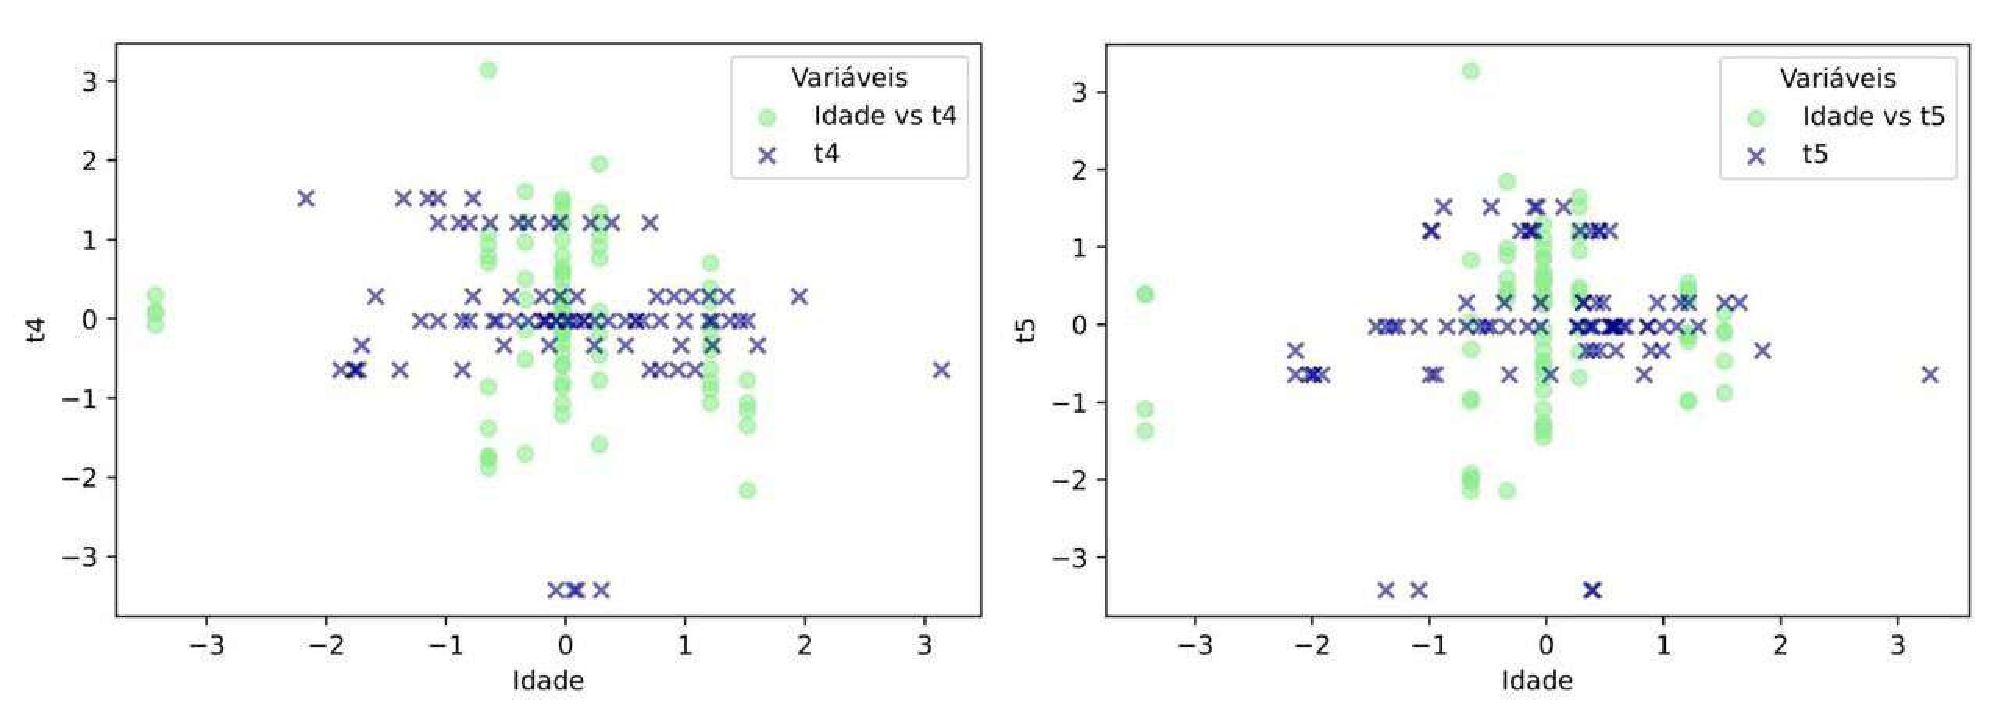
\includegraphics[scale=0.4]{figuras/Spearman/idade-t4-t5.pdf}
    \vspace{0.3cm} 
    \caption{A análise da dispersão entre Idade e as variáveis t4 e t5, utilizando o coeficiente de Spearman, revela correlações leves. O coeficiente de Spearman entre Idade e t4 foi de -0,15, indicando uma correlação monotônica negativa fraca, ou seja, à medida que a idade aumenta, há uma leve tendência de redução no tempo t4. Já entre Idade e t5, o coeficiente foi de 0,11, sugerindo uma correlação monotônica positiva fraca, indicando que o aumento da idade pode estar associado a um leve aumento no tempo t5.}
    \begin{minipage}{\linewidth}
        \centering
    \end{minipage}
\end{figure}
\FloatBarrier 

Ao reparar em alguns índices negativos, observamos os índices \textbf{tSB (-0.10), cc2 (t3-t2) (-0.17), s2 (t4-t3) (-0.24),  s3 (t8-t5) (-0.28) e a Ploidia(-0.50)}. Nota-se que os coeficientes mais próximos de 0 (como -0,10 a -0,28) indicam uma correlação negativa fraca. Isso traduz que há uma tendência muito sutil de que, quando uma variável aumenta, a idade, a outra diminui. Em \textit{tSB} Figura \ref{fig:idade-tSB-cc2-s2-s3}, o coeficiente negativo insinua que o tempo de formação inicial da blastocisto tende a ser menor em embriões provenientes de mães mais velhas. Na variável \textit{cc2}, Figura \ref{fig:idade-tSB-cc2-s2-s3}, a correlação desfavorável sugere uma maior irregularidade no intervalo entre a segunda e a terceira divisão celular (t2 para t3) em embriões de mães mais velhas. Em \textbf{s2} (Figura \ref{fig:idade-tSB-cc2-s2-s3}) e \textit{s3} (Figura \ref{fig:idade-tSB-cc2-s2-s3}), mostra que a idade materna também está ligada a uma diminuição na eficácia do intervalo entre as divisões celulares de t3 para t4. Isso indica um efeito na fase intermediária do ciclo celular. Nos embriões de mães mais velhas, o período entre a fase de 8 células e a formação do blastocisto final é estendido, sinalizando obstáculos no progresso dessas fases. Todos esses atrasos podem ser cruciais, já que fases iniciais bem sincronizadas são fundamentais para um desenvolvimento embrionário adequado, mostrando como uma idade avançada pode afetar o desenvolvimento embrionário, afirmando a bibliografia estudada, fato já citado por \citeonline{borges2019}, que reitera que \textbf{a idade materna exerce maior influência sobre a qualidade embrionária}.

\begin{figure}[h]
    \captionsetup{font=footnotesize, justification=centering, labelsep=period, position=above}
    \caption{Dispersão entre Idade e tSB - Coeficiente de Spearman: -0.10 | Dispersão entre Idade e cc2 (t3-t2) - Coeficiente de Spearman: -0.15 | Dispersão entre Idade e s2 (t4-t3) - Coeficiente de Spearman: -0.24 | Dispersão entre Idade e s3 (t8-t5) - Coeficiente de Spearman: -0.28}
    \label{fig:idade-tSB-cc2-s2-s3}
    \centering
    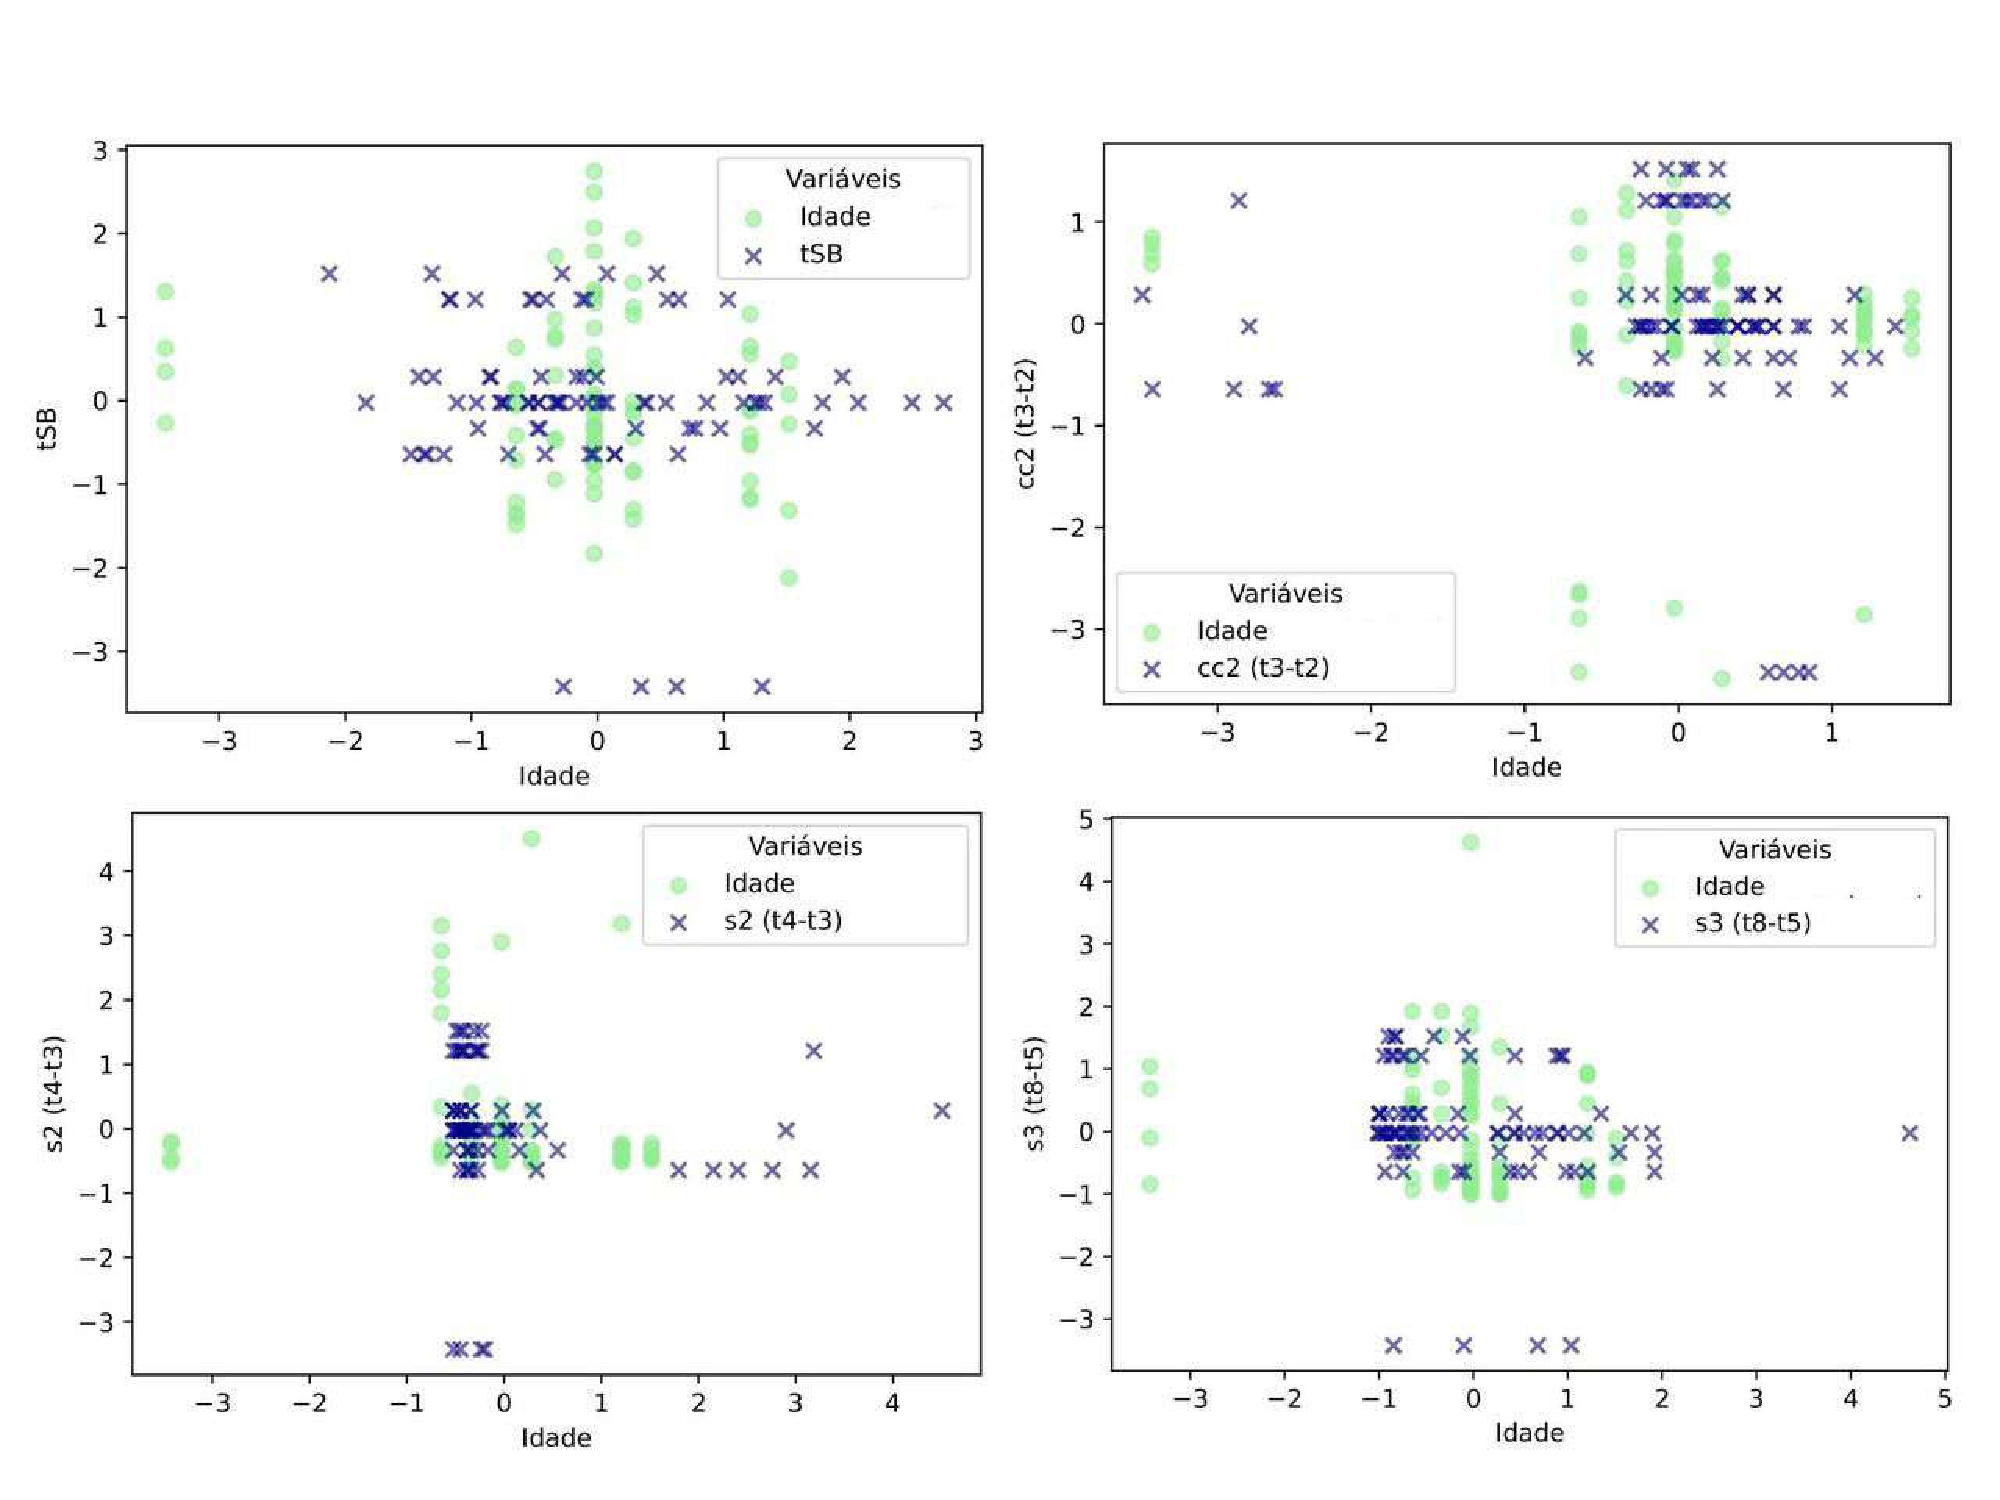
\includegraphics[scale=0.4]{figuras/Spearman/Idade-tSB_cc2_s2_s3.pdf}
    \vspace{0.3cm} 
    \caption{A análise das relações entre Idade e as variáveis tSB, cc2 (t3-t2), s2 (t4-t3) e s3 (t8-t5) revela correlações negativas de diferentes intensidades, sugerindo que o aumento da idade pode estar associado a uma redução nos respectivos intervalos de tempo. A correlação entre Idade e tSB (-0,10) e entre Idade e cc2 (t3-t2) (-0,15) é fraca, indicando uma leve tendência de diminuição desses valores com o aumento da idade, mas sem um padrão claro. Já a correlação entre Idade e s2 (t4-t3) (-0,24) é moderadamente negativa, sugerindo uma relação mais perceptível entre o aumento da idade e a redução desse intervalo. A relação mais intensa foi observada entre Idade e s3 (t8-t5) (-0,28), apontando que a idade pode influenciar de maneira mais consistente a redução desse tempo. }
    \begin{minipage}{\linewidth}
        \centering
    \end{minipage}
\end{figure}
\FloatBarrier

Analisando os índices positivos, temos \textbf{tB-tSB (0.20)} e \textbf{cc3 (t5-t3) (0.20)} com valores que sugerem que a elevação de uma variável está de forma sutil ligada ao crescimento da outra. Em relação ao intervalo entre o estágio de \textbf{cc3} (Figura \ref{fig:idade-cc3}) e \textbf{tB-tSB} (Figura \ref{fig:idade-tB-tSB}) nos embriões de mulheres mais velhas aumenta levemente. Este crescimento pode sugerir que, mesmo com atrasos em etapas posteriores, o embrião busca se ajustar para compensar o desenvolvimento inicial mais lento.

No gráfico de dispersão entre as variáveis Idade e tSB, se nota que o eixo Y, que simboliza a variável tSB, alcança valores próximos a 120. Esta característica está ligada à origem dos dados, onde o tSB varia de 81 a 127,7, enquanto a Idade se situa em uma escala mais limitada (28 a 44 anos). A diferença visual no gráfico é previsível e espelha fielmente os valores reais contidos na planilha, sem sinalizar qualquer erro.

\begin{figure}[h]
    \captionsetup{font=footnotesize, justification=centering, labelsep=period, position=above}
    \centering
    \begin{minipage}[b]{0.45\linewidth}
        \caption{Dispersão entre Idade e tB-tSB - Coeficiente de Spearman: 0.20}
        \label{fig:idade-tB-tSB}
        \centering
        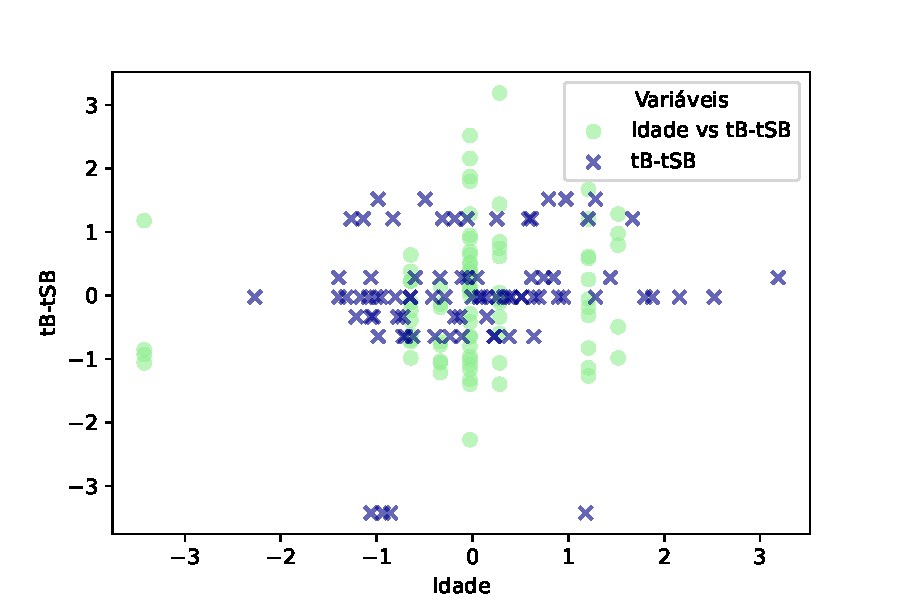
\includegraphics[scale=0.47]{figuras/Spearman/idade-tB-tSB.pdf}
        \vspace{0.3cm}
        \caption{Indica uma correlação monotônica positiva fraca. Isso sugere que, à medida que a idade aumenta, há uma leve tendência de aumento no intervalo tB-tSB, embora sem um padrão fortemente definido. }
        \begin{minipage}{\linewidth}
            \centering
        \end{minipage}
    \end{minipage}
    \hspace{0.05\linewidth}
    \begin{minipage}[b]{0.45\linewidth}
        \caption{Dispersão entre Idade e cc3 (t5-t3) - Coeficiente de Spearman: 0.20}
        \label{fig:idade-cc3}
        \centering
        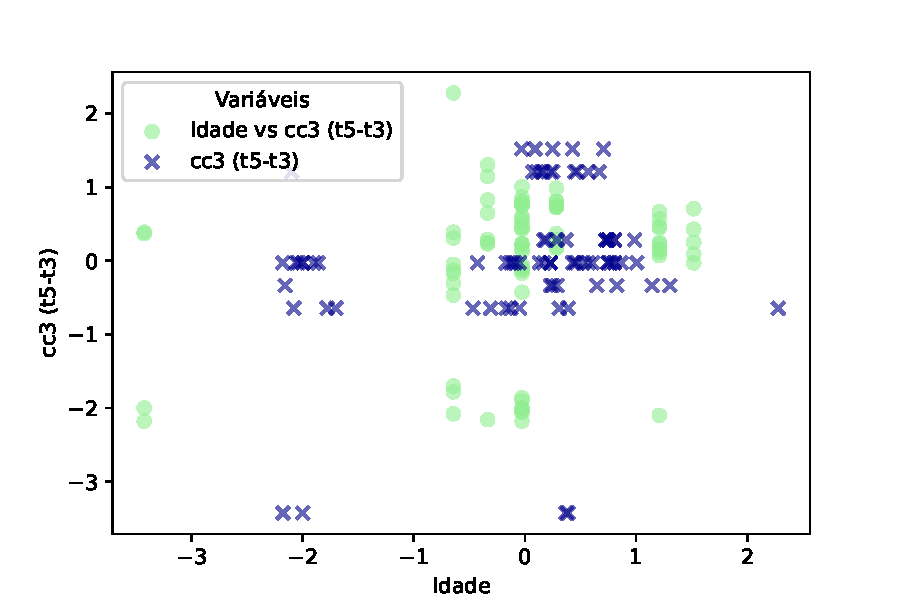
\includegraphics[scale=0.47]{figuras/Spearman/idade-cc3.pdf}
        \vspace{0.3cm}
        \caption{Indica uma correlação monotônica positiva fraca. Isso sugere que, com o aumento da idade, há uma leve tendência de aumento no intervalo cc3 (t5-t3), embora sem uma relação fortemente definida. }
        \begin{minipage}{\linewidth}
            \centering
        \end{minipage}
    \end{minipage}
\end{figure}
\FloatBarrier

E por fim temos a \textit{Ploidia (-0,50)}, a correlação negativa mais relevante entre todas as outras variáveis, que sugere uma relação negativa, demonstrando que \textbf{a alta idade materna está ligada a uma diminuição na proporção de embriões euploides. Esta informação indica que embriões de mães mais velhas contêm uma proporção reduzida de euploidia, o que pode estar ligado a uma queda na qualidade genética dos embriões}. Portanto, a idade materna é um dos elementos chave na diminuição da euploidia embrionária, alinhando com as informações de \textit{Fertility and Ageing} \cite{eshre2005}, que também reitera que o aumento da aneuploidia em embriões está diretamente associado ao envelhecimento materno.

\subsection*{Estágio}
Os coeficientes de correlação de Spearman entre os \textit{estágios} e os tempos de transição celular \textit{(t2, t3, t4, t5, t8)} revelam relações positivas moderadas. Esses dados indicam que, \textbf{conforme o embrião progride para estágios mais avançados, os tempos associados às divisões celulares iniciais tendem a aumentar de forma sutil}. Por exemplo, \textit{t2 (0,30), t3 (0,25) e t4 (0,32)} apresentam as correlações mais significativas, evidenciando que o avanço no estágio está vinculado a uma maior duração das transições celulares iniciais. Por outro lado, \textit{t5 (0,15) e t8 (0,17)}, apesar de apresentarem correlações mais baixas, também corroboram essa tendência de relação positiva. Esses resultados sugerem que o progresso do estágio embrionário está associado a um padrão de desenvolvimento, possivelmente, mais metódico nos estágios iniciais e intermediários do ciclo celular.

As correlações positivas observadas entre o \textit{estágio} embrionário e os tempos \textit{tSC (0,50), tSB (0,53) e tB (0,59)} indicam uma conexão significativa entre o progresso do estágio embrionário e o desenvolvimento contínuo das estruturas celulares. O incremento nos índices de correlação sugere que, conforme \textbf{o embrião avança para fases mais desenvolvidas, há uma maior regularidade no cumprimento dos marcos temporais dessas transições}. Isso implica que o estágio não apenas representa uma condição de desenvolvimento estrutural, mas também abriga informações significativas sobre a dinâmica temporal do ciclo celular. Assim, essas correlações ressaltam que o estágio embrionário atua como um indicador abrangente da qualidade e da evolução do desenvolvimento embrionário.

A relação inversa entre o \textit{estágio} de desenvolvimento e a \textit{ploidia (-0,24)} indica que, \textbf{embora essa correlação seja considerada tênue, sugere que o estágio de desenvolvimento pode ter um impacto negativo na ploidia}, enfatizando a necessidade de avaliar não apenas a morfologia do embrião, mas também sua genética ao longo do ciclo celular. 

\subsection*{Morfo}
A avaliação da variável \textit{Morfo}, que categoriza a expansão morfológica dos embriões em fases iniciais, revelou correlações moderadamente negativas com variáveis temporais como \textbf{t2 (-0.38), t3 (-0.43) e t5 (-0.45)}. Esses achados sugerem que \textbf{embriões com características morfológicas menos expansivas costumam apresentar atrasos nos primeiros tempos de divisão celular}. Assim, mudanças na morfologia podem ser influenciadas por variações no ritmo de desenvolvimento celular. Dessa forma, os dados estão alinhados com a literatura, que cita que a morfologia do embrião é um fator determinante para o potencial de implantação e a qualidade embrionária \citeonline{capalbo2014}.

Ao examinarmos os intervalos \textit{cc2 (t3-t2) (-0,38) e cc3 (t5-t3) (-0,31)}, os gráficos \ref{fig:morfo-cc2} e \ref{fig:morfo-cc3}, respectivamente, corroboram essa tendência, destacando que embriões que apresentam alterações morfológicas menos favoráveis quando enfrentam flutuações no ritmo de desenvolvimento celular, a medida que uma variável aumenta, a outra vem a diminuir. Esses resultados enfatizam a relevância de uma divisão celular sincronizada para preservar características morfológicas ideais, evidenciando como o ritmo do ciclo celular influencia diretamente a qualidade estrutural do embrião.

A correlação entre \textit{Morfo} e \textit{Ploidia} exibe um coeficiente de correlação de \textit{0.05}, sugerindo uma ligação positiva, porém extremamente fraca. Isso sugere que, neste conjunto de dados, as características morfológicas dos embriões não parecem estar diretamente ligadas à euploidia. 

\subsection*{t2, t3, t4, t5 e t8}
Existe uma forte interdependência entre os tempos de transição celular, como evidenciado pela correlação de \textit{0.89} entre \textit{t2 e t4}, indicando que esses eventos de desenvolvimento estão fortemente associados, à medida que uma variável aumenta, a outra também aumenta de forma consistente. A correlação entre \textit{t3 e t2 (0.78), t4 e t5 (0.56)} e entre \textit{t5 e t8 (0.52)} também demonstra alinhamento nas fases iniciais e intermediárias do desenvolvimento embrionário. 

\begin{figure}[h]
    \captionsetup{font=footnotesize, justification=centering, labelsep=period, position=above}
    \centering
    \begin{minipage}[b]{0.45\linewidth}
        \caption{Dispersão entre t2 e t4 - Coeficiente de Spearman: 0.89}
        \label{fig:t2-t4}
        \centering
        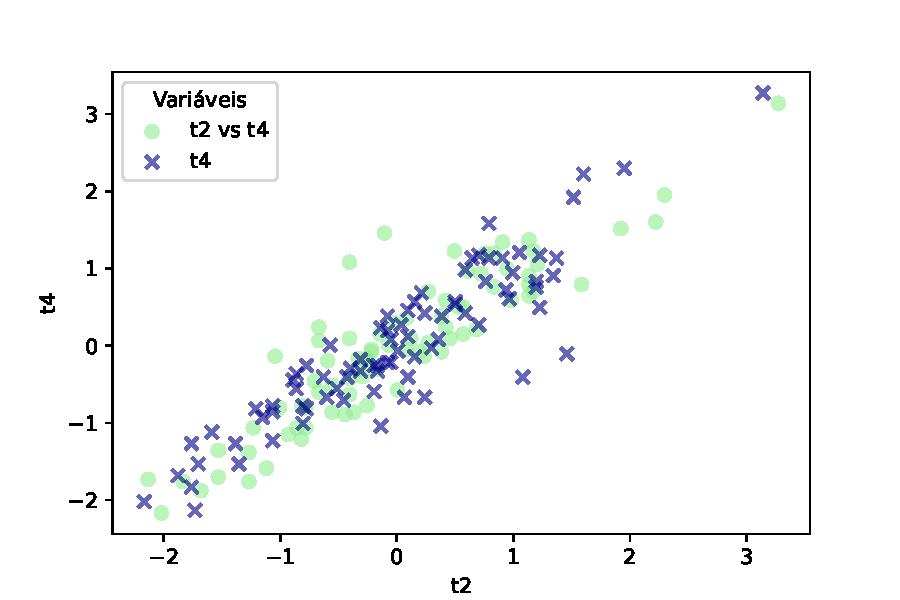
\includegraphics[scale=0.49]{figuras/Spearman/t2-t4.pdf}
        \vspace{0.3cm}
        \caption{Indica uma correlação monotônica positiva forte. Isso significa que, à medida que o valor de t2 aumenta, t4 também tende a aumentar de forma consistente.}
        \begin{minipage}{\linewidth}
            \centering
        \end{minipage}
    \end{minipage}
    \hspace{0.05\linewidth}
    \begin{minipage}[b]{0.45\linewidth}
        \caption{Dispersão entre t3 e t2 - Coeficiente de Spearman: 0.78}
        \label{fig:t3-t2}
        \centering
        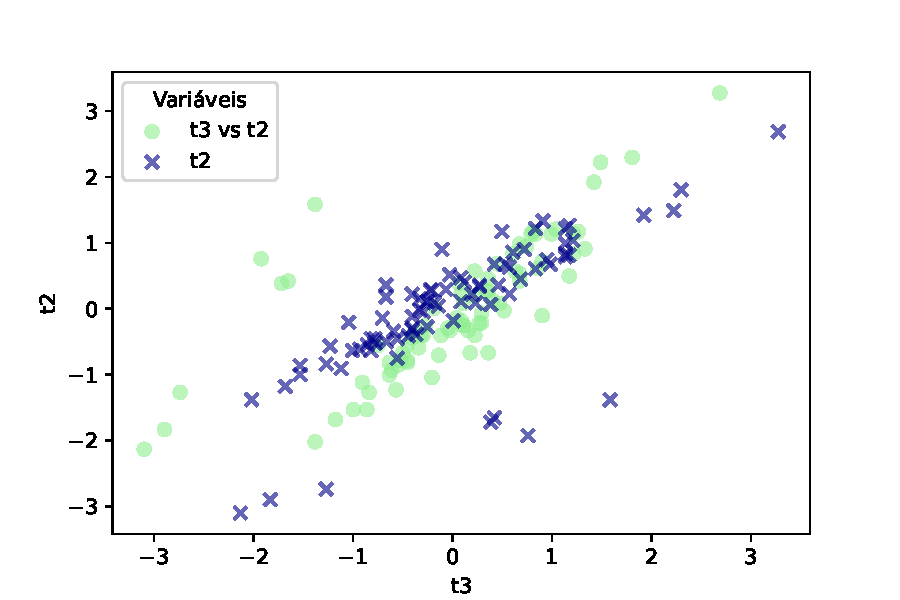
\includegraphics[scale=0.35]{figuras/Spearman/t3-t2.pdf}
        \vspace{0.3cm}
        \caption{Indica uma correlação monotônica positiva forte. Isso significa que, à medida que t2 aumenta, t3 também tende a aumentar de forma consistente, embora com uma relação um pouco menos intensa do que a observada entre t2 e t4.}
        \begin{minipage}{\linewidth}
            \centering
            \scriptsize{Fonte: Autoras (2025)}
        \end{minipage}
    \end{minipage}
\end{figure}
\FloatBarrier

\begin{figure}[h]
    \captionsetup{font=footnotesize, justification=centering, labelsep=period, position=above}
    \centering
    \begin{minipage}[b]{0.45\linewidth}
        \caption{Dispersão entre t4 e t5 - Coeficiente de Spearman: 0.56}
        \label{fig:t4-t5}
        \centering
        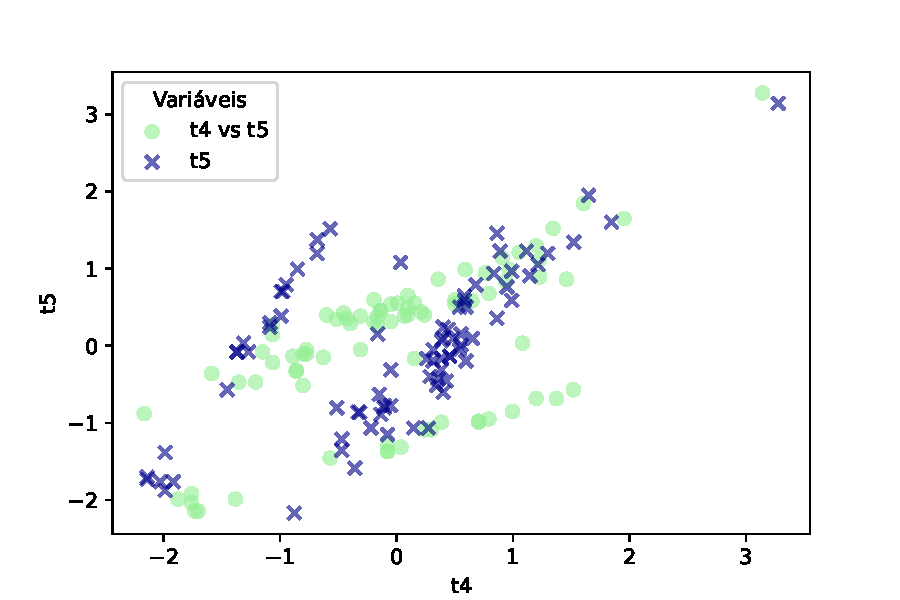
\includegraphics[scale=0.48]{figuras/Spearman/t4-t5.pdf}
        \vspace{0.3cm}
        \caption{Indica uma correlação monotônica positiva moderada. Isso significa que, à medida que t4 aumenta, t5 também tende a aumentar. Esse resultado sugere que o tempo necessário para atingir t5 está parcialmente influenciado pelo tempo t4}
        \begin{minipage}{\linewidth}
            \centering
        \end{minipage}
    \end{minipage}
    \hspace{0.05\linewidth}
    \begin{minipage}[b]{0.45\linewidth}
        \caption{Dispersão entre t5 e t8 - Coeficiente de Spearman: 0.52}
        \label{fig:t5-t8}
        \centering
        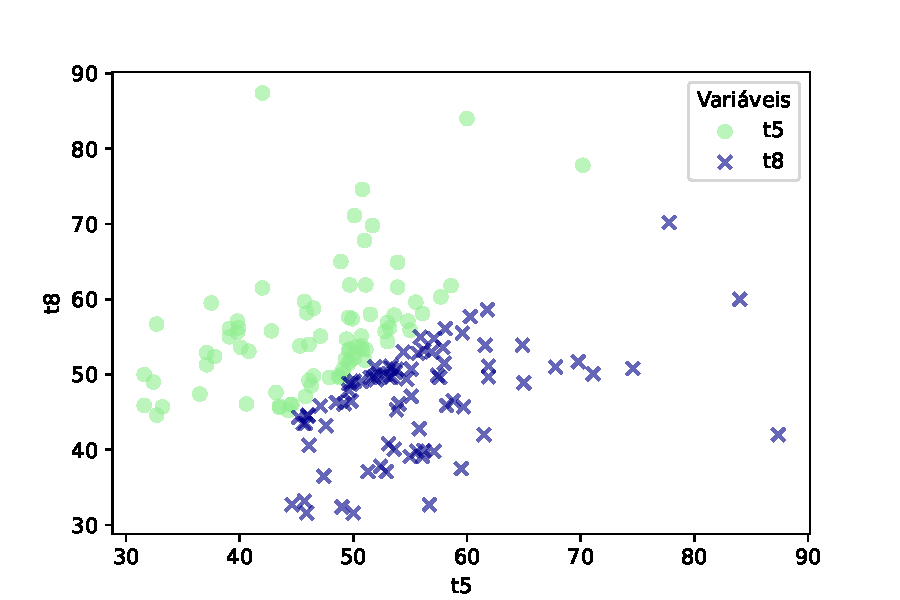
\includegraphics[scale=0.48]{figuras/Spearman/t5-t8.pdf}
        \vspace{0.3cm}
        \caption{Indica uma correlação monotônica positiva moderada. Isso sugere que, à medida que t5 aumenta, t8 também tende a aumentar. Essa correlação sugere uma dependência entre esses dois tempos}
        \begin{minipage}{\linewidth}
            \centering
        \end{minipage}
    \end{minipage}
\end{figure}
\FloatBarrier

A correlação quase nula entre \textit{t2 (-0.08), t3 (-0.06), t4 (-0.02), t8 (-0.07) e a ploidia}, demonstram uma falta de correlação entre essas variáveis para a determinação de um embrião euploidia ou aneuplóide. Já \textbf{\textit{t5} e \textit{ploidia (-0.24)} indica que atrasos nesse estágio de desenvolvimento, estão ligados a uma qualidade genética inferior (menor ploidia)}, alinhando com a literatura, que destaca t5 como o indicador mais relevante do potencial de implantação \citeonline{cruz2012}. 

\subsection*{tSC}
Ao relacionar a variável de Tempo de formação do estágio de clivagem sincronizada (Time to Synchronized Compaction) com as variáveis de tempos de transição celular, \textit{t2 (0.40), t3 (0.42), t4 (0.43), t5 (0.35) e t8 (0.35)}, indicam uma relação de intensidade moderada e positiva durante o desenvolvimento embrionário, sendo mais acentuada nos estágios iniciais e intermediários. A conexão com \textit{t2}, Figura \ref{fig:tSC-t2}, sugere uma interdependência inicial que persiste em \textit{t3}, Figura \ref{fig:tSC-t3}, e se intensifica um pouco em \textit{t4}, Figura \ref{fig:tSC-t4}, indicando um alinhamento mais intenso nas etapas intermediárias do ciclo celular. As correlações com \textit{t5 e t8}, Figura \ref{fig:tSC-t8}, apresentam uma ligeira redução, sugerindo que o impacto do \textit{tSC} nos eventos embrionários começa a se desvanecer em fases mais avançadas. Esses padrões indicam que o \textbf{tSC tem um papel mais significativo nas etapas iniciais e intermediárias do desenvolvimento, diminuindo seu impacto progressivamente conforme o tempo passa}. 

\begin{figure}[h]
    \captionsetup{font=footnotesize, justification=centering, labelsep=period, position=above}
    \centering
    \begin{minipage}[b]{0.45\linewidth}
        \caption{Dispersão entre tSC e t2 - Coeficiente de Spearman: 0.40}
        \label{fig:tSC-t2}
        \centering
        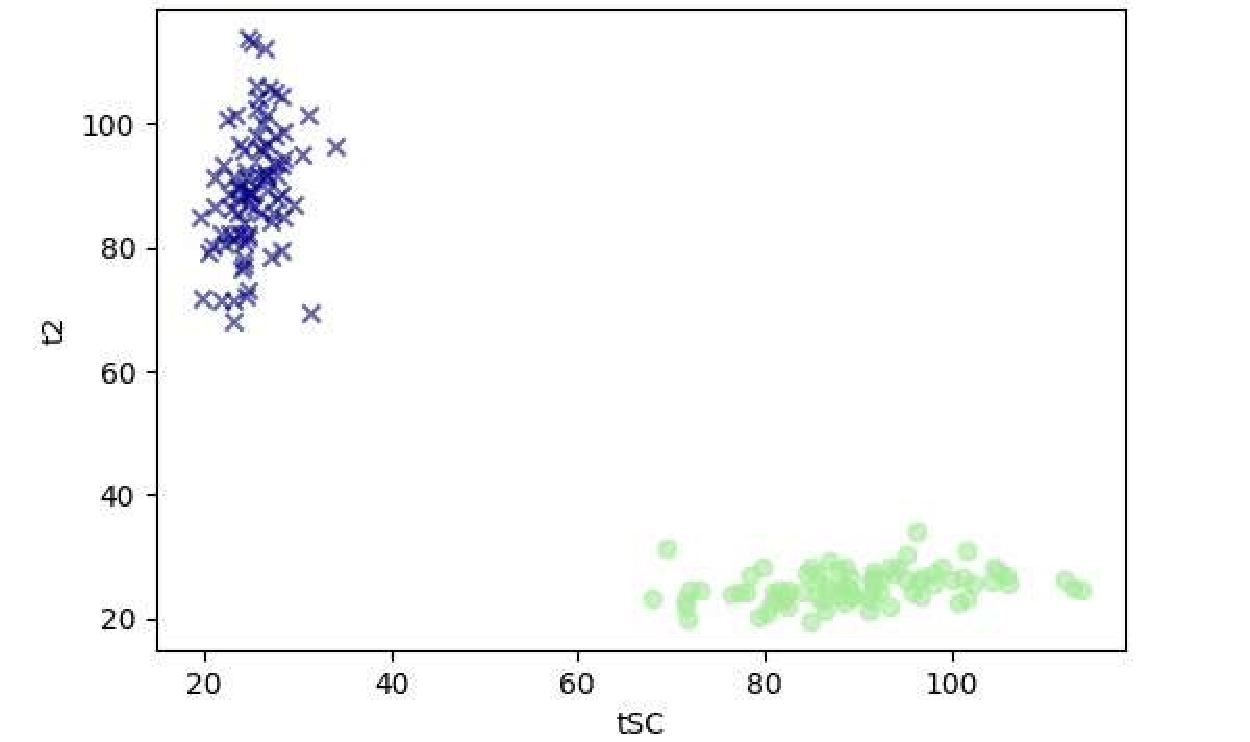
\includegraphics[scale=0.35]{figuras/Spearman/tSC-t2.pdf}
        \vspace{0.3cm}
        \caption{A análise da dispersão entre tSC e t2, com um coeficiente de Spearman de 0,40, revela uma correlação positiva moderada. Existe  uma tendência para que tSC aumente à medida que t2 aumenta. Esse valor sugere que a associação entre tSC e t2 é perceptível.}
        \begin{minipage}{\linewidth}
            \centering
        \end{minipage}
    \end{minipage}
    \hspace{0.05\linewidth}
    \begin{minipage}[b]{0.45\linewidth}
        \caption{Dispersão entre tSC e t3 - Coeficiente de Spearman: 0.42}
        \label{fig:tSC-t3}
        \centering
        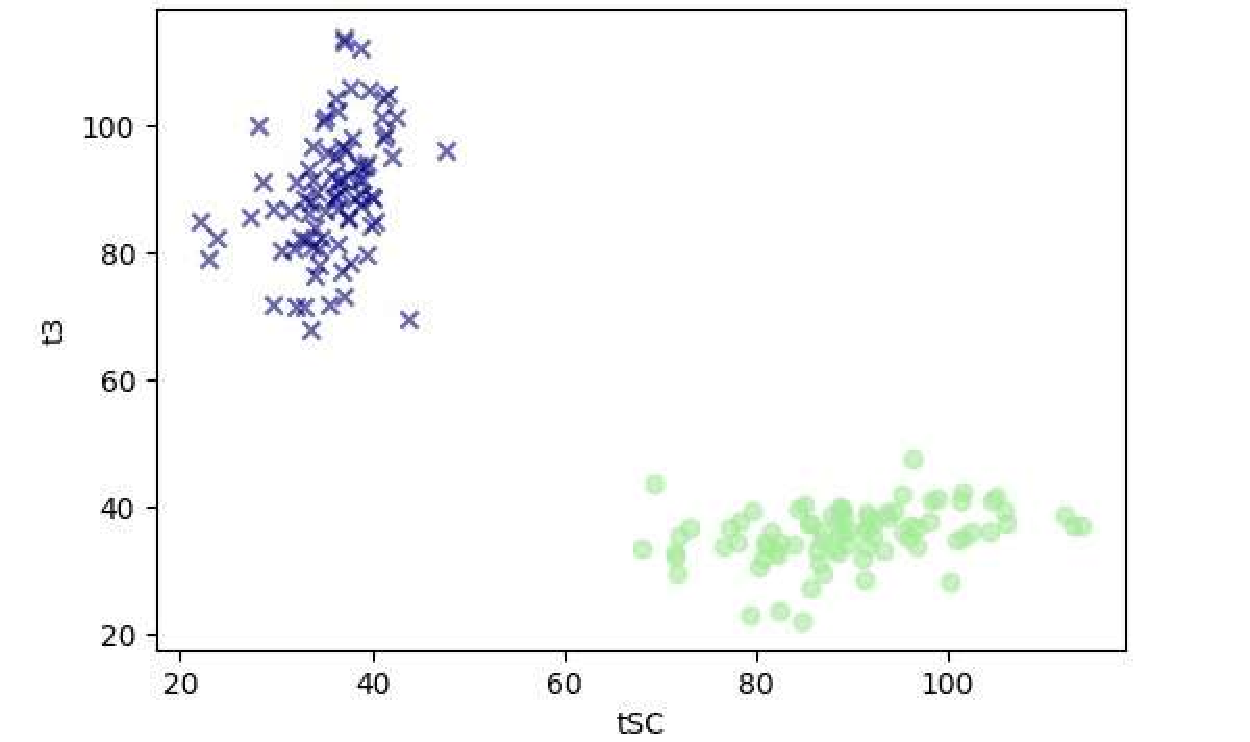
\includegraphics[scale=0.35]{figuras/Spearman/tSC-t3.pdf}
        \vspace{0.3cm}
        \caption{A análise da dispersão entre tSC e t3, com um coeficiente de Spearman de 0,42, indica uma correlação positiva moderada entre esses tempos embrionários. Isso sugere que, à medida que o tempo t3 avança, o tempo tSC também tende a aumentar.}
        \begin{minipage}{\linewidth}
            \centering
        \end{minipage}
    \end{minipage}
\end{figure}
\FloatBarrier

\begin{figure}[h]
    \captionsetup{font=footnotesize, justification=centering, labelsep=period, position=above}
    \centering
    \begin{minipage}[b]{0.45\linewidth}
        \caption{Dispersão entre tSC e t4 - Coeficiente de Spearman: 0.43}
        \label{fig:tSC-t4}
        \centering
        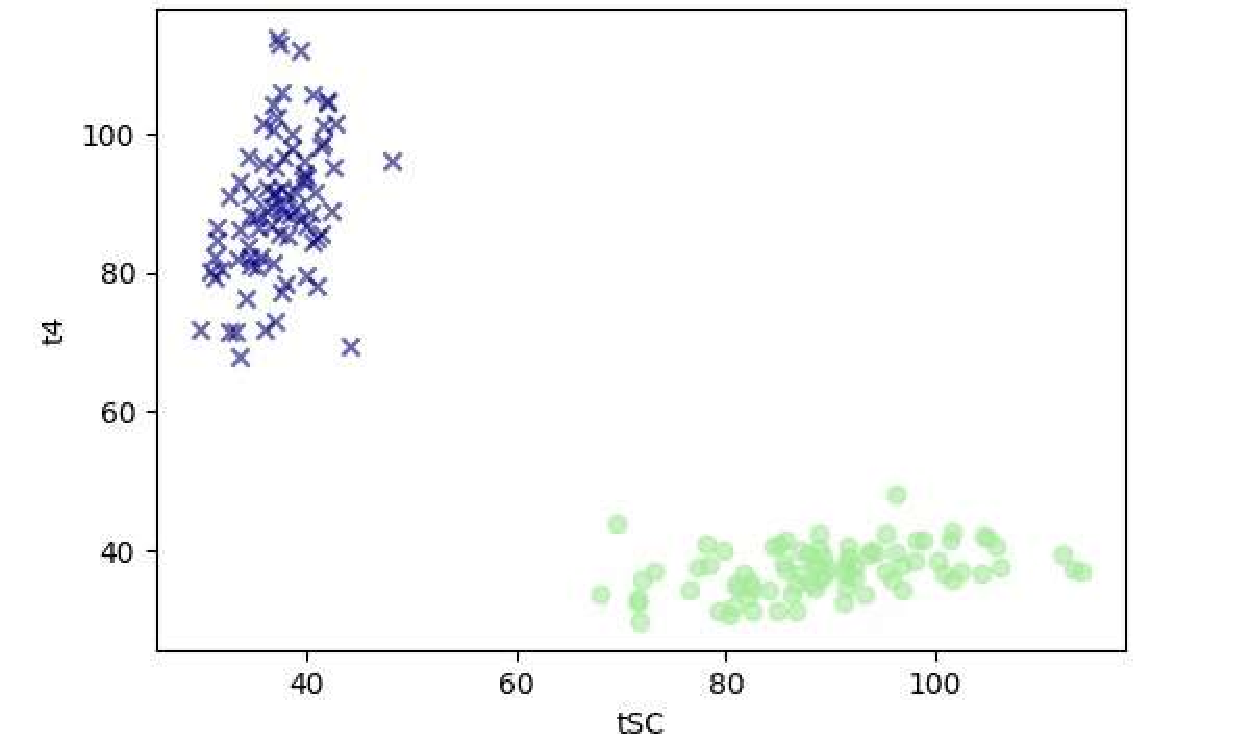
\includegraphics[scale=0.35]{figuras/Spearman/tSC-t4.pdf}
        \vspace{0.3cm}
        \caption{A análise da dispersão entre tSC e t4, com um coeficiente de Spearman de 0,43, revela uma correlação positiva moderada entre esses dois tempos embrionários. Isso indica que essa correlação sugere que existe uma certa tendência de sincronização entre esses estágios do desenvolvimento embrionário.}
        \begin{minipage}{\linewidth}
            \centering
        \end{minipage}
    \end{minipage}
    \hspace{0.05\linewidth}
    \begin{minipage}[b]{0.45\linewidth}
        \caption{Dispersão entre tSC e t8 - Coeficiente de Spearman: 0.35}
        \label{fig:tSC-t8}
        \centering
        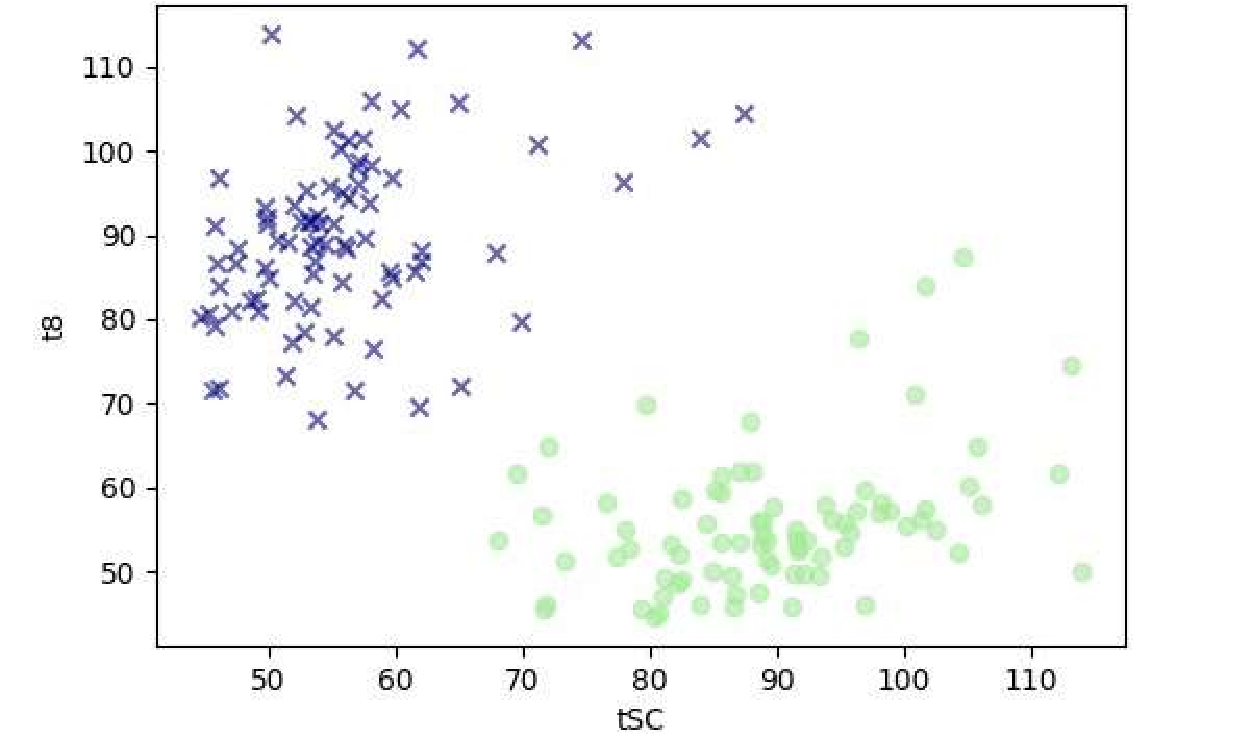
\includegraphics[scale=0.35]{figuras/Spearman/tSC-t8.pdf}
        \vspace{0.3cm}
        \caption{Indica uma correlação positiva moderada, embora relativamente fraca. Essa correlação pode refletir uma tendência de associação no desenvolvimento embrionário, porém, devido à sua moderação.}
        \begin{minipage}{\linewidth}
            \centering
        \end{minipage}
    \end{minipage}
\end{figure}
\FloatBarrier

As correlações de \textit{tSC} com \textit{tSB (0.75) e tB (0.74)}, Figura \ref{fig:tSC-tSB} e Figura \ref{fig:tSC-tB} respectivamente, demonstram uma forte ligação entre essas variáveis, indicando que estão fortemente conectadas, em que a medida que uma variável aumenta, a outra também aumenta de forma consistente. Isso indica uma relação quase linear, em que mudanças no tSB impactam diretamente no tSC, evidenciando uma ligação funcional direta entre os dois acontecimentos. A variável tSC permanece sendo identificada pelo marcador “o” nos gráficos a seguir.

\begin{figure}[h]
    \captionsetup{font=footnotesize, justification=centering, labelsep=period, position=above}
    \centering
    \begin{minipage}[b]{0.45\linewidth}
        \caption{Dispersão entre tSC e tSB - Coeficiente de Spearman: 0.75}
        \label{fig:tSC-tSB}
        \centering
        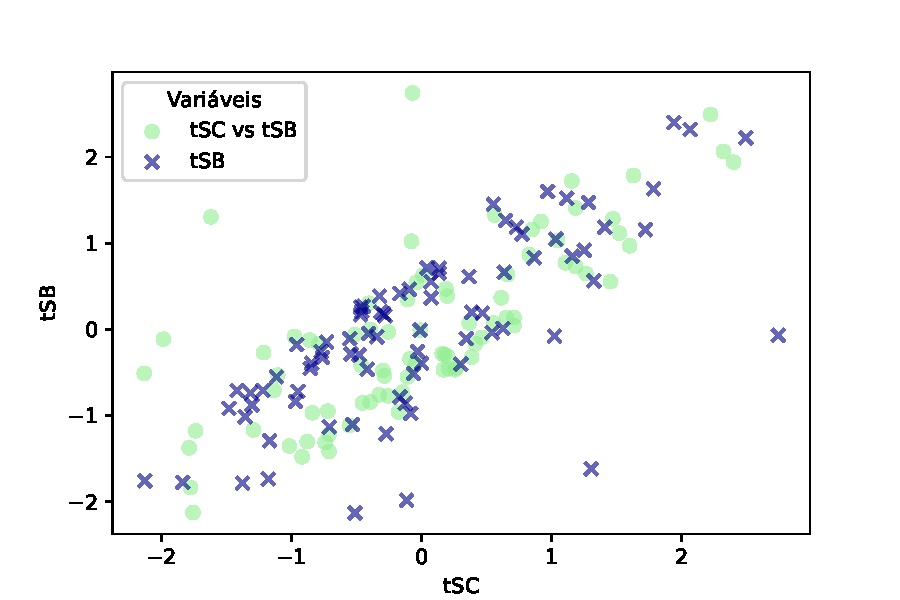
\includegraphics[scale=0.35]{figuras/Spearman/tSC-tSB.pdf}
        \vspace{0.3cm}
        \caption{A alta correlação entre essas duas variáveis sugere que há uma relação significativa entre elas no desenvolvimento embrionário, indicando que o tempo tSB pode ser um fator importante no comportamento do tempo tSC.}
        \begin{minipage}{\linewidth}
            \centering
            \scriptsize{Fonte: Autoras (2025)}
        \end{minipage}
    \end{minipage}
    \hspace{0.05\linewidth}
    \begin{minipage}[b]{0.45\linewidth}
        \caption{Dispersão entre tSC e tB - Coeficiente de Spearman: 0.74}
        \label{fig:tSC-tB}
        \centering
        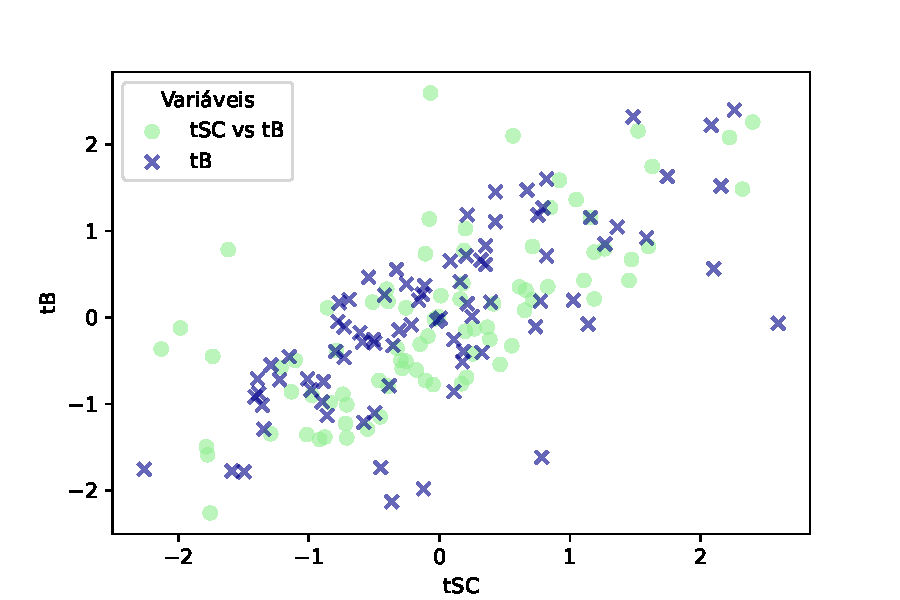
\includegraphics[scale=0.35]{figuras/Spearman/tSC-tB.pdf}
        \vspace{0.3cm}
        \caption{Há uma tendência clara de que, conforme tB aumenta, tSC também se eleva, sugerindo que essas duas variáveis estão fortemente associadas no contexto do desenvolvimento embrionário. }
        \begin{minipage}{\linewidth}
            \centering
            \scriptsize{Fonte: Autoras (2025)}
        \end{minipage}
    \end{minipage}
\end{figure}
\FloatBarrier

Os coeficientes de correlação de tSC com os intervalos de tempo \textit{cc2 (t3-t2) (0.41), cc3 (t5-t3) (0.24) e t5-t2 (0.34)} apresentam relações positivas que variam de moderadas a fracas, sinalizando variados níveis de concordância com esses tempos acumulados. A correlação moderada com \textit{cc2 (t3-t2)} indica que o intervalo entre t3 e t2 tem uma influência moderada no tSC, evidenciando uma ligação mais clara neste estágio. Em contrapartida, a correlação fraca com \textit{cc3 (t5-t3)} sugere que as alterações no intervalo entre \textbf{t5 e t3} exercem uma influência restrita sobre o tSC. Por outro lado, a relação moderada com \textit{t5-t2} indica que o tempo acumulado entre esses eventos afeta o tSC, embora em menor grau do que com cc2. Estes achados indicam que a influência do tSC se \textbf{reduz} conforme os períodos de tempo se estendem.

Por fim, a correlação com a \textit{Ploidia (-0.04)}, é fraca e negativa, sugerindo que não existe uma conexão relevante entre essas variáveis. Este resultado indica que Ploidia pode estar ligada a processos diferentes que não afetam diretamente \textit{tSC}.

\subsection*{tSB}
Ao analisar sua realção com \textit{t2 (0.43), t3 (0.56), t4 (0.57), t5 (0.39) e t8 (0.40)} mostram relações positivas de intensidade moderada, conforme uma variável aumenta, a outra segue um aumento consistente, aumentando nos estágios iniciais e intermediários e apresentando um ligeiro declínio nos estágios posteriores. A relação com \textit{t2} \textbf{indica que os eventos iniciais exercem um efeito significativo no comportamento de \textbf{tSB}}. A forte ligação com \textit{t3 e t4}, Figura \ref{fig:tSB-t3} e Figura \ref{fig:tSB-t4} respectivamente, indica que \textbf{esses estágios intermediários têm uma influência mais significativa sobre \textbf{tSB}}. Em contrapartida, as correlações moderadas com \textbf{t5 e t8} sugerem uma redução na conexão nos estágios subsequentes, evidenciando um efeito menos significativo de \textit{tSB} conforme os processos progridem no desenvolvimento.

As correlações entre \textit{tSB e tSC (0.75), tB (0.93) e cc2 (t3-t2) (0.63)} evidenciam ligações fortes e relevantes, indicando uma interdependência entre essas variáveis. A forte ligação com \textbf{tSC} sugere que alterações em uma variável têm um \textbf{impacto direto} na outra. \textbf{A correlação com tB indica uma dependência quase total entre as duas variáveis}, indicando que são praticamente comparáveis em termos de sua interação. Ademais, a correlação robusta com cc2 (t3-t2) indica que \textbf{o período entre t3 e t2 tem um impacto considerável sobre tSB, possivelmente por causa do efeito direto dos eventos temporais iniciais no comportamento dessa variável}. A Figura \ref{fig:tSB-tB} ilustra a forma que \textit{tSB e tB} possuem uma relação de crescimento mútuo entre si, quase se espelhando. Dessa forma, alterações em tB podem ser significativas para mudanças em tSB.

\begin{figure}[h]
    \captionsetup{font=footnotesize, justification=centering, labelsep=period, position=above}
    \caption{Dispersão entre tSB e tB - Coeficiente de Spearman: 0.93}
    \label{fig:tSB-tB}
    \centering
    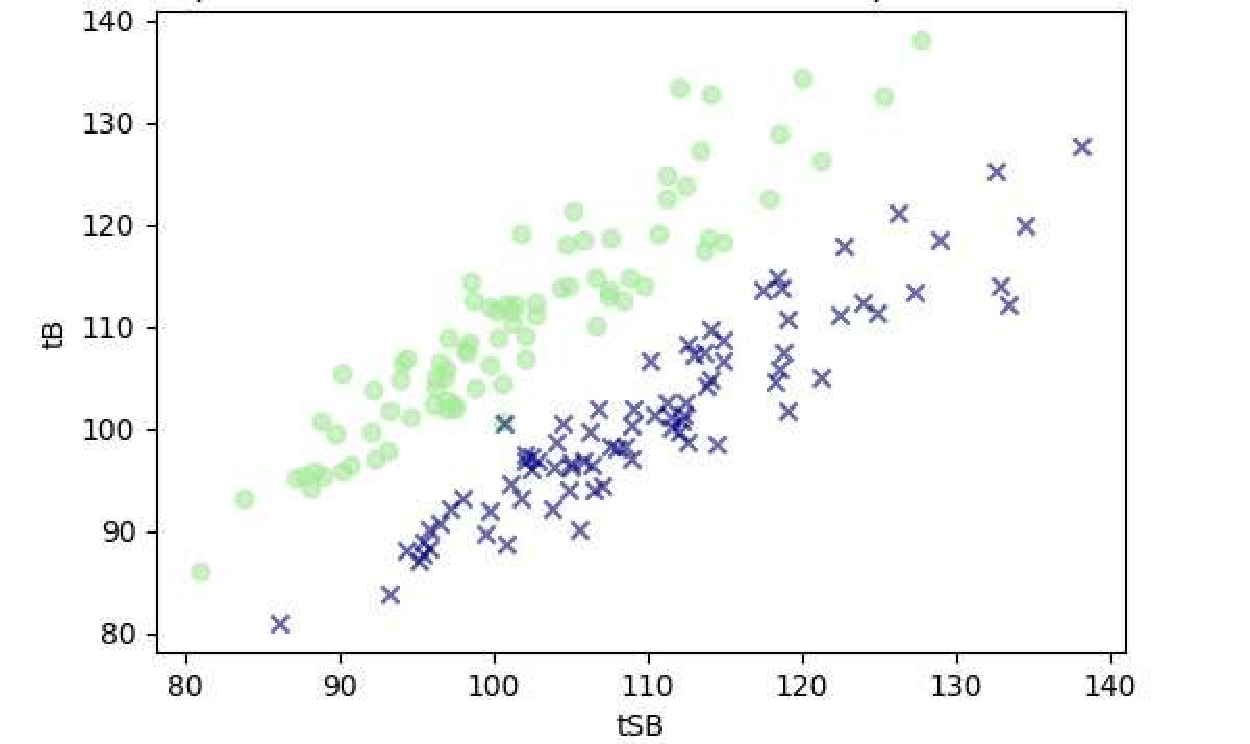
\includegraphics[scale=0.40]{figuras/Spearman/tSB-tB.pdf}
    \vspace{0.3cm} 
    \caption{A análise da dispersão entre tSB e tB, com um coeficiente de Spearman de 0,93, revela uma correlação positiva extremamente forte. Isso indica que, à medida que tB aumenta, tSB também tende a aumentar de maneira quase perfeitamente sincronizada.}
    \begin{minipage}{\linewidth}
        \centering
    \end{minipage}
\end{figure}
\FloatBarrier

O coeficiente de correlação de \textit{tSB com Ploidia (-0.11)} é fraco e negativo, sugerindo que não existe uma conexão evidente ou relevante entre essas variáveis. Este resultado indica que Ploidia é afetada por elementos diferentes, que não estão diretamente ligados aos processos ligados à tSB.

\subsection*{tB}
As correlações entre \textit{tB} e os tempos de desenvolvimento \textit{t2 (0.40), t3 (0.48), t4 (0.50), t5 (0.35) e t8 (0.37)} exibem relações moderadamente positivas, sugerindo que tB está ligado a eventos temporais durante o ciclo embrionário, sendo mais intensa nos estágios intermediários. A forte ligação com \textit{t3 e t4} sugere que tB está mais em sintonia com eventos desses estágios, o que pode indicar uma interação mais intensa com processos de divisão celular intermediários. O crescimento da correlação em \textit{t4} pode indicar uma etapa crucial para o desenvolvimento do embrião. Por outro lado, as correlações mais baixas com \textit{t5 e t8} indicam uma redução da influência do tB em fases mais avançadas, ressaltando que sua importância é maior nos estágios iniciais e intermediários do ciclo celular.

As correlações de tB com os intervalos de tempo \textit{cc2 (t3-t2) (0.54) e tSC-t8 (0.47)} ressaltam a influência de processos particulares no comportamento dessa variável. A correlação moderada-alta com \textit{cc2 (t3-t2)} indica que \textbf{os períodos de transição entre t3 e t2 têm uma influência relevante no comportamento de tB}, sugerindo que as dinâmicas nos estágios iniciais influenciam diretamente o desenvolvimento subsequente. Em contrapartida, a correlação moderada entre \textit{tSC e t8} indica que a diferença temporal entre \textbf{tSC e t8} está positivamente ligada a tB. 

A fraca e negativa correlação entre \textit{tB e Ploidia (-0.17)} indica uma conexão fraca entre essas variáveis. A direção negativa sugere que aumentos em tB podem estar ligados a pequenas diminuições em Ploidia. Esta associação tênue enfatiza que tB não desempenha um papel crucial no comportamento da Ploidia, porém o afeta fracamente de forma negativa.

\subsection*{cc2 (t3-t2)}
A relação entre o intervalo \textit{cc2} e as diversas fases de crescimento do embrião, simbolizadas pelos tempos \textit{t2, t3, t4, t5 e t8}, mostra variações de intensidade. A correlação com \textit{t2 (0.39)} é moderada e positiva, indicando que acontecimentos iniciais, como o surgimento das primeiras células embrionárias, possuem uma ligação direta, porém não tão relevante com cc2. Com \textit{t3 (0.80)}, se nota, na figura \ref{fig:cc2-t3}, uma correlação positiva significativa, demonstrando um \textbf{alinhamento quase imediato entre cc2} e o momento de desenvolvimento correspondente a \textit{t3}, sugerindo uma \textbf{conexão robusta entre ambos}. Por outro lado, a correlação com \textbf{t4 (0.59)} é moderadamente alta, indicando que \textbf{cc2 é também impactado por eventos subsequentes representados por t4}. A conexão com t5 (0.64), também moderada-alta, \textbf{evidencia a persistência da influência de eventos temporais}, evidenciando que t5 desempenha um papel significativo na progressão de cc2. Por fim, com t8 (0.46), a correlação é moderada, porém o efeito de t8 sobre cc2 é menos significativo do que nos estágios anteriores, \textbf{sugerindo uma dependência que diminui conforme o embrião progride para fases mais avançadas de desenvolvimento}. O gráfico abaixo mostra a maior relação que cc2 possui durante as fases de crescimento, que é na fase \textbf{t3 (0.80)}, em que a variável cc2 (t3-t2), cresce de forma consistente à medida que a outra também cresce. 

\begin{figure}[h]
    \captionsetup{font=footnotesize, justification=centering, labelsep=period, position=above}
    \caption{Dispersão entre cc2 (t3-t2) e t3 - Coeficiente de Spearman: 0.80}
    \label{fig:cc2-t3}
    \centering
    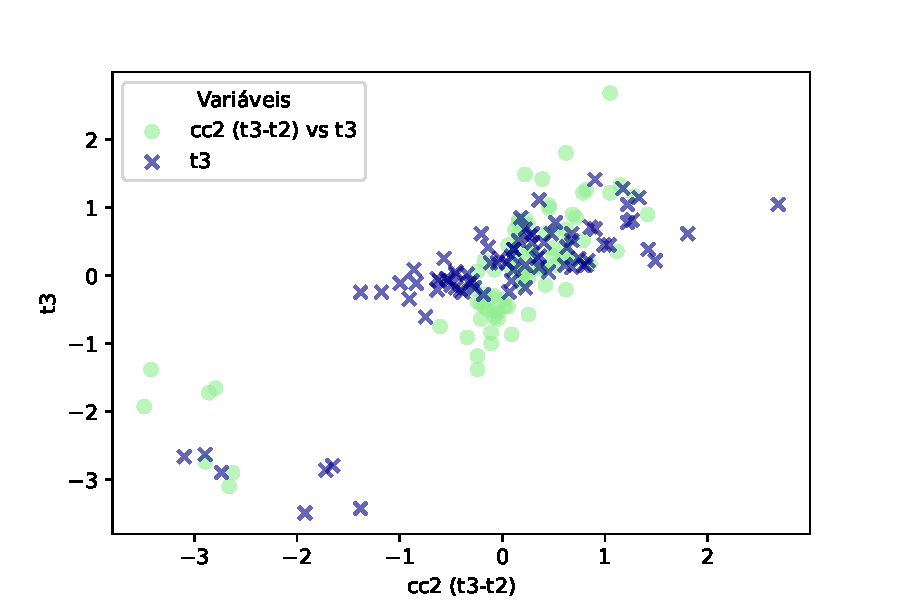
\includegraphics[scale=0.4]{figuras/Spearman/cc2-t3.pdf}
    \vspace{0.3cm} 
    \caption{A alta correlação entre essas variáveis sugere que o tempo t3 tem uma influência considerável sobre o intervalo cc2, refletindo uma associação significativa no desenvolvimento embrionário. }
    \begin{minipage}{\linewidth}
        \centering
    \end{minipage}
\end{figure}
\FloatBarrier

A correlação com \textit{cc3 (0.34)} é moderada, sugerindo uma relação restrita entre cc2 e cc3. Por outro lado, a correlação com \textit{t5-t2 (0.65)} é forte e positiva, indicando que o intervalo \textit{cc2 se alinha fortemente ao intervalo completo entre t5 e t2}. Isso indica que o comportamento de cc2 pode ser significativamente elucidado pela combinação das variáveis que compõem esses intervalos de tempo, evidenciando uma relação mais sólida entre eles.

A correlação entre \textit{cc2 e Ploidia (-0.03)} é muito fraca e negativa, sugerindo que não existe uma conexão relevante entre esses dois componentes. Isso indica que \textbf{o período temporal entre t3 e t2 não tem um impacto significativo na Ploidia}, o que sugere que o desenvolvimento temporal do embrião, simbolizado por cc2, não está diretamente ligado à ploidia do embrião.

\subsection*{cc3 (t5-t3)}
A correlação com \textit{t2 (0.15)} é fraca e positiva, sugerindo que pequenas alterações em t2 não provocam alterações significativas em cc3. Com \textit{t3 (0.25)}, a correlação é moderada e positiva, mostrando um ligeiro crescimento em cc3 à medida que t3 se eleva. A correlação com \textit{t4 (0.26)} é igualmente moderada e positiva. A conexão entre t4 e cc3 é parecida com a de t3, porém um pouco mais intensa, indicando que t4 desempenha um papel moderado nas alterações percebidas em cc3. A correlação com \textit{t5 (0.81)}, presente na figura \ref{fig:cc3-t5}, é extremamente forte e positiva, sugerindo que \textbf{conforme t5 cresce, cc3 também cresce quase de maneira linear}, como se consegue observar no gráfico abaixo, em que cc3 está definido pelo marcador “o”. Isso é coerente, já que cc3 é determinado como a diferença entre t5 e t3, e qualquer alteração em t5 afeta diretamente cc3. Por fim, a correlação com o \textbf{t8 (0.40)} é moderada e positiva, indicando que, conforme o t8 se eleva, o cc3 tende a crescer. O t8 tem um impacto maior sobre o cc3 do que o t2, t3, e t4, mas ainda distante do impacto de t5.

A correlação entre o intervalo \textit{t5-t3 (representado por cc3)} e o intervalo \textit{t5-t2 (0.90)} é extremamente forte e positiva como pode ser visto na figura \ref{fig:cc3-t5-t2}, \textbf{sugerindo que o comportamento de cc3 está fortemente ligado ao intervalo t5-t2}. Isso corrobora a noção de que as alterações de t5 em relação a outras variáveis temporais, como t2, têm um impacto significativo em cc3. Portanto, o intervalo t5-t2 pode ser um indicador relevante para prever o comportamento de cc3, indicando que \textbf{a evolução do embrião entre os estágios t5 e t2 desempenha um papel relevante no comportamento de cc3 (t5-t3)}. Isso indica que alterações nesse intervalo temporal afetam significativamente a diferença de tempo entre os estágios t5 e t3. 

A correlação entre cc3 e o intervalo \textit{s3 (-0.36)} é moderada e negativa, sugerindo que conforme s3 se eleva, a tendência é que cc3 diminua. Esta correlação indica que um \textbf{aumento no intervalo entre t8 e t5 pode estar inversamente ligado a alterações em cc3}, o que poderia indicar um comportamento de compensação entre as variáveis. Ao estender o tempo entre os estágios t8 e t5, pode haver uma diminuição no comportamento observado em cc3 (t5-t3), indicando uma interação entre esses momentos de desenvolvimento do embrião.

A correlação de cc3 com a \textit{Ploidia (-0.281)} é bastante elevada quando comparada a outras variáveis, como a correlação de Ploidia com t2 (-0.075) ou t5 (-0.237). Isso sugere que \textbf{cc3 exerce uma influência moderada e negativa sobre a Ploidia, indicando que alterações na cc3 podem ter um impacto mais relevante sobre a ploidia do que em outras variáveis temporais}. Este efeito adverso indica que alterações em cc3 estão ligadas a uma diminuição no valor da ploidia. No entanto, \textbf{a correlação entre cc3 e Ploidia é evidente}, indicando uma influência mais significativa em relação a outras variáveis temporais.

\subsection*{t5-t2}
A correlação com \textit{Morfo (-0.38)} é moderadamente negativa, sugerindo que, conforme o valor de Morfo cresce, o intervalo t5-t2 tende a se estreitar. Isso indica que \textbf{as características morfológicas do embrião podem influenciar o comportamento temporal entre os estágios t5 e t2}, possivelmente indicando um desenvolvimento mais devagar ou desordenado conforme as características morfológicas se modificam.

Com \textit{t2 (0.21)}, a correlação é fraca e positiva, sugerindo uma pequena ligação entre o crescimento de t2 e o intervalo t5-t2, porém essa relação é pouco relevante. Com \textit{t3 (0.51)}, a correlação é moderada e positiva, sugerindo uma correlação mais intensa entre os intervalos temporais dos estágios t5 e t3. A correlação com \textit{t4 (0.39)} também é moderada e positiva, embora um pouco menos intensa que com t3, sugerindo que t4 também afeta o intervalo entre t5 e t2, porém em uma escala menor. Com \textit{t5 (0.92)}, a correlação é extremamente intensa e positiva, sinalizando que \textbf{o período entre t5 e t2 está fortemente ligado ao tempo de t5. Isso é esperado, pois t5 representa o término desse intervalo}. A correlação robusta indica que \textbf{alterações em t5 afetam consideravelmente o intervalo entre t5 e t2}. A correlação com \textit{t8 (0.45)} é positiva e moderada, indicando uma conexão entre t8 e o intervalo t5-t2, embora não seja tão intensa quanto com t5.

Com \textit{tSB (0.40) e tB (0.37)}, as correlações são moderadas e positivas, indicando que \textbf{a mudança nos tempos tSB e tB também afeta o intervalo entre t5 e t2}. No caso de \textit{s3 (indicado por t8-t5, -0.41)}, a correlação é moderada e negativa, indicando que, \textbf{conforme o intervalo t8-t5 cresce, o intervalo t5-t2 tende a se reduzir, indicando um possível comportamento compensatório entre os dois períodos de tempo}.

O coeficiente de correlação de \textbf{Ploidia (-0.23)} com t5-t2 é moderado e negativo, sugerindo \textbf{uma relação inversa entre as alterações na ploidia e o intervalo entre t5 e t2}. Isso indica que, \textbf{conforme t5-t2 evolui, a ploidia tende a se reduzir, indicando uma possível restrição da ploidia no comportamento temporal entre esses estágios}. 

\subsection*{s2 (t4-t3)}
A correlação com \textit{t3 (-0.22)} é moderada e negativa, sugerindo que conforme o valor de t3 cresce, a distância s2 (t4-t3) tende a se afilar. Isso indica que uma alteração no tempo t3 pode diminuir a distância entre t4 e t3, sugerindo que as alterações no tempo t3 estão um pouco inversamente ligadas a esse intervalo. A correlação de \textit{t4 (0.16)} é fraca e positiva, indicando uma pequena ligação entre o aumento de t4 e o intervalo s2 (t4-t3). 

A correlação com \textit{cc2 (t3-t2) (-0.21)} é moderada e negativa. Isso pode sugerir uma relação inversa entre o comportamento temporal dos intervalos t4-t3 e t3-t2, com alterações em cc2 impactando negativamente o intervalo s2, possivelmente por causa de um comportamento mais rápido no começo do desenvolvimento do embrião.

Com uma correlação moderada e positiva de \textit{s3 (t8-t5) (0.25)}, indica que um crescimento no intervalo s3 está ligado a um crescimento no intervalo s2. Isso pode sugerir que \textbf{o aumento do intervalo entre t8 e t5 está ligado ao aumento do intervalo entre t4 e t3}, o que pode representar uma compensação nos tempos entre as diversas fases do embrião.

A correlação com \textit{Ploidia (0.11)} é leve e positiva, sugerindo que alterações em s2 exercem um efeito levemente positivo na ploidia. Apesar do efeito ser mínimo, ele propõe que \textbf{uma alteração em s2 pode levar a uma pequena alteração na ploidia}.

\subsection*{s3 (t8-t5)}
A correlação com \textit{t5 (-0.39)} é moderada e negativa. Isso indica que \textbf{o período entre t8 e t5 diminui à medida que o estágio t5 progride, sugerindo que uma elevação em t5 pode levar a uma aceleração do progresso}, reduzindo o intervalo subsequente até t8. 

Com \textit{t8 (0.48)} na Figura \ref{fig:s3-t8}, a correlação é positiva e moderada mais alta que t5, indicando que, conforme t8 se eleva, o intervalo s3 também tende a se expandir. Isso sugere que um aumento no intervalo de tempo entre t8 e t5 está ligado a um incremento no valor de t8, sinalizando um processo de evolução mais extenso ou mais lento em comparação com outros intervalos. \textbf{Este resultado indica que, conforme o embrião se aproxima do estágio t8, o período de tempo entre os estágios t8 e t5 aumenta}, assim demonstrado no gráfico abaixo, em que s3 está em ver claro. 

\begin{figure}[h]
    \captionsetup{font=footnotesize, justification=centering, labelsep=period, position=above}
    \caption{Dispersão entre s3 (t8-t5) e t8 - Coeficiente de Spearman: 0.48}
    \label{fig:s3-t8}
    \centering
    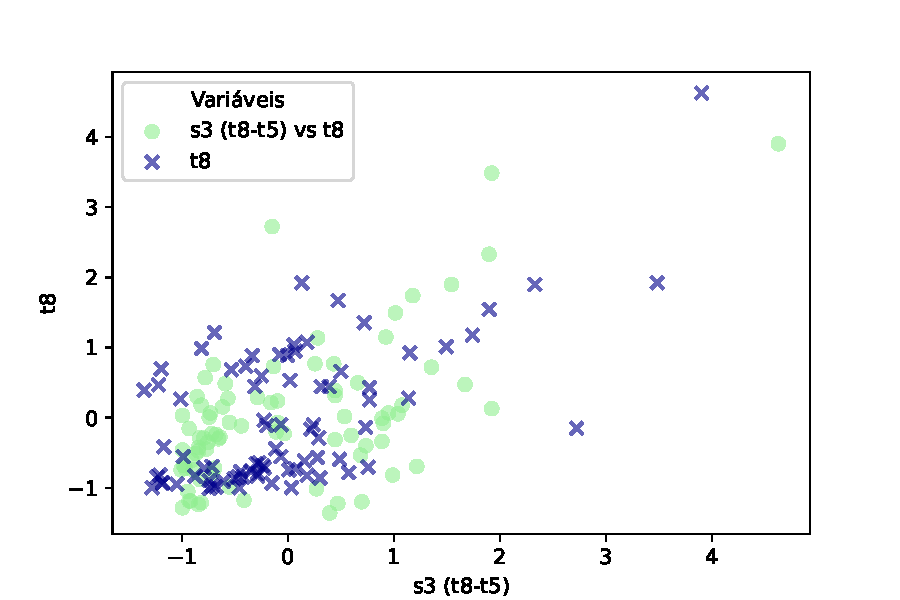
\includegraphics[scale=0.4]{figuras/Spearman/s3-t8.pdf}
    \vspace{0.3cm} 
    \caption{A correlação moderada entre essas duas variáveis indica que há uma associação entre elas, embora outros fatores possam estar influenciando essa relação.}
    \begin{minipage}{\linewidth}
        \centering
    \end{minipage}
\end{figure}
\FloatBarrier

A correlação com \textit{cc3 (t5-t3) (-0.36)} é moderada e negativa. Este efeito indica que uma extensão prolongada entre t5 e t3 pode estar ligada a uma diminuição no tempo entre t8 e t5, sugerindo que \textbf{o progresso no período intermediário (t5-t3) pode impactar diretamente os estágios finais}, acelerando o período entre t5 e t8.

A correlação com \textit{tSC-t8 (-0.35)} é moderada e negativa. Isso indica uma \textbf{relação de compensação entre as fases intermediárias e finais do desenvolvimento embrionário}, onde o tempo entre tSC e t8 diminui, enquanto o tempo entre t8 e t5 aumenta.

Finalmente, a correlação com a \textit{Ploidia (0.25)} é moderada e positiva, indicando que, conforme a ploidia cresce, o intervalo s3 (t8-t5) também tende a se expandir. Este efeito pode sugerir que a \textbf{aneuploidia está ligado a uma diminuição no tempo de desenvolvimento, estendendo o intervalo entre t8 e t5}. Este comportamento pode indicar variações no crescimento celular devido à composição genética do embrião, onde \textbf{aneuploidias podem resultar em um desenvolvimento mais lento}.

\subsection*{tSC-t8}
A relação com \textit{t8 (-0.29)} é moderadamente negativa sugere que, conforme o intervalo de tempo entre tSC e t8 cresce, o tempo de t8 também tende a crescer. Este resultado indica que,\textbf{ ao aumentar o intervalo entre tSC e t8, pode ocorrer uma diminuição na velocidade do desenvolvimento embrionário entre tSC e t8, estendendo o período até t8}. Isso pode indicar uma etapa de crescimento mais lenta ou prolongada, influenciando o ritmo geral de avanço do embrião.

A correlação com \textit{tSC (0.70)} é forte e positiva, que indica que o intervalo tSC-t8 tem uma ligação direta com o intervalo tSC. \textbf{Conforme o intervalo de tempo entre tSC e t8 se amplia, o intervalo tSC também tende a se expandir}. Isso mostra uma relação em que o começo do estágio tSC afeta diretamente o tempo entre tSC e t8, indicando que um intervalo mais extenso entre tSC e t8 pode ser parcialmente determinado pela duração do estágio tSC em si. \textbf{Este efeito indica uma relação temporal na qual o estágio tSC desempenha um papel significativo no progresso do embrião no período subsequente até t8}.

Em \textit{tSB (0.44)}, a correlação é moderadamente positiva e sugere que, conforme o intervalo tSB se amplia, o intervalo tSC-t8 também tende a crescer. Isso pode sugerir que o período entre tSB e tSC pode estar ligado a um prolongamento até t8, o que poderia sinalizar a continuidade do desenvolvimento embrionário em um estágio mais prolongado. Este resultado indica que\textbf{ um período mais extenso entre tSB e tSC pode se estender até o intervalo tSC-t8, estendendo o processo}.

A correlação de \textit{tB-tSB (0.20)} é positiva e indica que um crescimento no intervalo entre tB e tSB pode estar estreitamente ligado a um crescimento no intervalo tSC-t8. Isso indica que o avanço do desenvolvimento embrionário de tB para tSB pode afetar o intervalo de tempo entre tSC e t8, embora não de maneira tão marcante.

A correlação muito tênue \textit{(0.04)} e positiva sugere que Ploidia exerce uma influência mínima no intervalo tSC-t8. 

\subsection*{tB-tSB}
A correlação com a \textit{Idade (0.20)} sendo positiva e fraca indica que, conforme a idade avança, o intervalo tB-tSB também tende a crescer, mesmo que de maneira sutil. Isso pode sugerir que a idade da paciente pode ter um pequeno impacto no desenvolvimento embrionário, possivelmente indicando uma variação no ritmo de desenvolvimento.

A correlação moderadamente positiva do \textit{Estágio (0.38)} indica que, conforme o estágio de desenvolvimento progride, o intervalo tB-tSB tende a se estender. Este efeito sugere que \textbf{fases mais avançadas do desenvolvimento embrionário podem estar ligadas a um prolongamento no intervalo entre tB e tSB}, o que pode indicar um avanço mais lento ou um intervalo mais extenso entre os eventos celulares que caracterizam tais fases.

A correlação moderadamente positiva de \textit{tB (0.38)} indica que, conforme o intervalo tB se amplia, o intervalo tB-tSB também tende a se expandir. Isso é coerente, já que \textbf{o período tB é um estágio inicial do desenvolvimento embrionário, e sua duração pode impactar diretamente o tempo até o estágio seguinte}, o tSB, impactando a evolução do desenvolvimento embrionário. Uma maior extensão do tB geralmente indica um período mais extenso até o tSB.

A correlação de \textit{tSC-t8 (0.20)} é fraca e positiva correlação sugere uma pequena ligação entre o intervalo tB-tSB e o intervalo tSC-t8. Isso indica que alterações no intervalo tB-tSB podem estar ligadas a alterações no tempo entre tSC e t8, mesmo que essa conexão seja restrita. 

A correlação com \textit{Ploidia (-0.284)} exerce um efeito significativo, visto que \textbf{é a segunda correlação de maior magnitude entre as variáveis examinadas}. Desempenha um papel significativo, uma vez que indica que a qualidade genética do embrião, avaliada por tB e tSB, pode impactar diretamente a ploidia. Isso pode ser interpretado como um sinal de que \textbf{embriões com predisposições genéticas mais favoráveis, tais como ploidia euploide ou mosaico de baixo grau, podem exibir um ritmo acelerado de desenvolvimento, evidenciado pelo intervalo mais breve entre essas fases cruciais do seu desenvolvimento}. Essa correlação negativa sugere que a qualidade genética não só afeta a saúde do embrião, mas também pode influenciar a temporização dos eventos celulares. 

\subsection*{Ploidia}
A avaliação das variáveis relacionadas à ploidia indica que \textbf{a idade materna tem o maior efeito na qualidade genética do embrião}. A idade materna, \textbf{com uma correlação de -0,50}, apresenta uma correlação inversa significativa com a ploidia. Isso significa que, \textbf{conforme a mulher envelhece, a quantidade de embriões euploides diminui, o que indica um crescimento na taxa de aneuploidia}. Isso está alinhado com o que a literatura já aponta sobre o impacto do envelhecimento materno na qualidade genética dos embriões, onde embriões de mulheres mais idosas têm maior probabilidade de conter erros cromossômicos. Assim, a idade materna é um elemento crucial na avaliação da ploidia embrionária e deve ser levada em conta em procedimentos de fertilização in vitro.

Adicionalmente, as variáveis \textbf{tB-tSB e cc3 (t5-t3)} possuem uma correlação moderada de -0,28 com a ploidia, sugerindo que o período entre as fases de desenvolvimento \textbf{t5, t3, tB e tSB podem afetar diretamente a qualidade genética do embrião}. Este intervalo de tempo está ligado ao ritmo de divisão celular e ao comportamento dos cromossomos. Mudanças nesse processo podem comprometer a criação de embriões euploides, levando a um aumento na probabilidade de aneuploidia. Essa correlação sugere que a sincronização adequada do desenvolvimento embrionário entre esses estágios é fundamental para a formação de embriões geneticamente saudáveis.

Outros fatores, como o \textbf{estágio de desenvolvimento (-0,24) e o t5 (-0,24)}, também mostraram uma correlação negativa com a ploidia. Isso indica que \textbf{o avanço para fases mais avançadas de desenvolvimento e o atraso no t5 podem estar ligados a uma queda na qualidade genética dos embriões}. Essas variáveis enfatizam a necessidade de um acompanhamento exato do desenvolvimento embrionário, pois pequenas mudanças no intervalo entre as fases podem influenciar o comportamento genético do embrião, levando a embriões com menor probabilidade de implantação.

\subsubsection{Atividade 4 (A4): Separar o conjunto de dados em conjuntos de treinamento, validação e teste, fazendo uma distribuição dos dados e aplicar técnica de aumento de dados}
Nessa atividade, apresentamos a implementação do procedimento de segmentação do conjunto de dados em três subconjuntos diferentes: treinamento, validação e teste. Esta distribuição obedece às proporções estabelecidas na metodologia (70\%, 15\% e 15\%, respectivamente) e foi feita através de um \textit{script} em Python. Utilizamos a planilha criada pela Atividade 1, a ``\texttt{Planilha\_normalizada.xlsx}'', pois utilizaremos os dados já normalizados e tratados a partir de agora.

A segmentação do conjunto de dados foi planejada para assegurar que cada subconjunto tenha uma representação adequada para seus respectivos propósitos, com já citado na Capítulo 3 em Metodologia. A distribuição foi feita de maneira aleatória para prevenir viés e assegurar a aplicabilidade geral do modelo. O \textit{script} calculou o tamanho de cada subconjunto com base em um total 82 linhas de amostra, seguindo as porcentagens estabelecidas.

Através do código, garantimos que os conjuntos produzidos sejam apropriados para as fases seguintes de treinamento, validação e teste do modelo de IA, mantendo a integridade dos dados originais.

\subsection*{Arquivos Gerados}
Os conjuntos de dados foram convertidos em arquivos Excel, cada um denominado conforme sua função. Cada subconjunto reflete a diversidade presente no conjunto original e o embaralhamento garante que os subconjuntos não compartilhem padrões específicos devido à ordenação prévia dos dados.

\subsection*{Aumento de Dados (\textit{Data Augmentation}) utilizando o Método de Monte Carlo:} 
A técnica de aumento de dados (\textit{data augmentation}) foi utilizada para melhorar o desempenho do modelo ao gerar mais exemplos de treinamento a partir dos dados existentes. Este processo visa aumentar a capacidade de generalização do modelo e evitar o \textit{overfitting}, tornando-o mais robusto.

O programa emprega distribuições estatísticas autênticas para produzir novas amostras que seguem os padrões dos dados originais. A distinção entre dados numéricos e categóricos possibilita o tratamento adequado de cada variável, garantindo a integridade do conjunto de dados ampliado.

A aplicação da média e do desvio padrão assegura que os novos dados numéricos correspondam às características do conjunto original, ao mesmo tempo que as categorias mantêm suas proporções, mantendo os padrões originais. A produção de dados por meio de distribuições estatísticas amplia a diversidade do conjunto sem adicionar ruído excessivo ou padrões inverossímeis, assegurando uma diversificação controlada. Este procedimento garante que o conjunto de treinamento ampliado seja robusto o suficiente para treinar o modelo, prevenindo sobrecargas e aprimorando a generalização, levando a um modelo mais eficiente e seguro.

Depois de executar o código, a quantidade de dados de treinamento foi triplicada, de acordo com o fator de ampliação estabelecido, utilizado em situações onde o conjunto de dados inicial é extremamente pequeno. O programa produziu novos valores numéricos através da distribuição normal, usando a média e o desvio padrão das colunas originais, assegurando que os novos valores preservassem as propriedades estatísticas do conjunto original. Por outro lado, as colunas categóricas tiveram seus valores replicados de forma aleatória, mantendo as proporções originais e a disposição das categorias. Esta operação resultou na geração de 228 linhas, o que equivale a três vezes o total de linhas existentes no conjunto de dados.